%%% The main file. It contains definitions of basic parameters and includes all other parts.

%% Settings for single-side (simplex) printing
% Margins: left 40mm, right 25mm, top and bottom 25mm
% (but beware, LaTeX adds 1in implicitly)
\documentclass[12pt,a4paper]{report}
\setlength\textwidth{145mm}
\setlength\textheight{247mm}
\setlength\oddsidemargin{15mm}
\setlength\evensidemargin{15mm}
\setlength\topmargin{0mm}
\setlength\headsep{0mm}
\setlength\headheight{0mm}
% \openright makes the following text appear on a right-hand page
\let\openright=\clearpage

%% Settings for two-sided (duplex) printing
% \documentclass[12pt,a4paper,twoside,openright]{report}
% \setlength\textwidth{145mm}
% \setlength\textheight{247mm}
% \setlength\oddsidemargin{14.2mm}
% \setlength\evensidemargin{0mm}
% \setlength\topmargin{0mm}
% \setlength\headsep{0mm}
% \setlength\headheight{0mm}
% \let\openright=\cleardoublepage

%% Generate PDF/A-2u
\usepackage[a-2u]{pdfx}

%% Character encoding: usually latin2, cp1250 or utf8:
\usepackage[utf8]{inputenc}

%% Prefer Latin Modern fonts
\usepackage{lmodern}

%% Further useful packages (included in most LaTeX distributions)
\usepackage{amsmath}        % extensions for typesetting of math
\usepackage{amssymb}
\usepackage{amsfonts}       % math fonts
\usepackage{amsthm}         % theorems, definitions, etc.
\usepackage{bm}             % boldface symbols (\bm)
\usepackage{graphicx}       % embedding of pictures
\usepackage{fancyvrb}       % improved verbatim environment
\usepackage{natbib}         % citation style AUTHOR (YEAR), or AUTHOR [NUMBER]
\usepackage[nottoc]{tocbibind} % makes sure that bibliography and the lists
			    % of figures/tables are included in the table
			    % of contents
\usepackage{dcolumn}        % improved alignment of table columns
\usepackage{booktabs}       % improved horizontal lines in tables
\usepackage{paralist}       % improved enumerate and itemize
\usepackage{xcolor}         % typesetting in color
\usepackage{parskip}		% indentation and space between paragraphs
\usepackage{caption}		% caption formatting
\usepackage[T1]{fontenc}	% font encoding
\usepackage[most]{tcolorbox}
\usepackage{fancyvrb}
\usepackage{relsize}
\usepackage{algpseudocode}
\usepackage{acro}

\newcommand\verbbf[1]{\textbf{#1}}
\newcommand\verbun[1]{\underline{#1}}
\newcommand\verbit[1]{\textit{#1}}
\newcommand\verbxs[1]{\small{\small{#1}}}

\tcbuselibrary{skins,breakable}
\newtcolorbox{mybox}[2][]{breakable,sharp corners, skin=enhancedmiddle jigsaw,parbox=false,
boxrule=0mm,leftrule=2mm,boxsep=0mm,arc=0mm,outer arc=0mm,attach title to upper,
after title={\ }, coltitle=black,colback=gray!10,colframe=black, title={#2},
fonttitle=\bfseries,#1}

%%% Basic information on the thesis

% Thesis title in English (exactly as in the formal assignment)
\def\ThesisTitle{Social network analysis in academic environment}

% Author of the thesis
\def\ThesisAuthor{Jindřich Bär}

% Year when the thesis is submitted
\def\YearSubmitted{2024}

% Name of the department or institute, where the work was officially assigned
% (according to the Organizational Structure of MFF UK in English,
% or a full name of a department outside MFF)
\def\Department{Department of Software Engineering}

% Is it a department (katedra), or an institute (ústav)?
\def\DeptType{Department}

% Thesis supervisor: name, surname and titles
\def\Supervisor{prof. RNDr. Tomáš Skopal, Ph.D.}

% Supervisor's department (again according to Organizational structure of MFF)
\def\SupervisorsDepartment{Department of Software Engineering}

% Study programme and specialization
\def\StudyProgramme{Computer Science}
\def\StudyBranch{Software and Data Engineering}

% An optional dedication: you can thank whomever you wish (your supervisor,
% consultant, a person who lent the software, etc.)
\def\Dedication{%
I would like to express my gratitude to prof. RNDr. Tomáš Skopal, PhD., for his scholarly leadership 
and for the time and advice he has given me during the writing of this thesis. 
I would also like to extend my thanks to my family and friends, who have supported and encouraged me 
greatly during my studies.
}

% Abstract (recommended length around 80-200 words; this is not a copy of your thesis assignment!)
\def\Abstract{
While university information systems usually have detailed data about courses, publication and lecturers, 
they rarely mine the relationships between these entities to provide additional value to the users.
In this thesis, we aim to improve the Charles Explorer web application by utilizing the synthesized academic social network from the existing relational data.
We propose a pipeline for transforming relational data from the university systems into a graph representation of the academic social network. 
We explore the network and propose various ways of utilizing the graph model for inferring missing data. 
Later, we benchmark different re-ranking strategies using the social network metrics against existing academic search engines and show that the social network-based re-ranking can improve the search results ranking.
Lastly, we reimplement the tool for visualising the academic social network in the Charles Explorer application for better user experience.
}

% 3 to 5 keywords (recommended), each enclosed in curly braces
\def\Keywords{%
{social network,} {academia,} {information retrieval,} {reranking}
}

%% The hyperref package for clickable links in PDF and also for storing
%% metadata to PDF (including the table of contents).
%% Most settings are pre-set by the pdfx package.
\hypersetup{unicode}
\hypersetup{breaklinks=true}

% Definitions of macros (see description inside)
%%% This file contains definitions of various useful macros and environments %%%
%%% Please add more macros here instead of cluttering other files with them. %%%

%%% Minor tweaks of style

% These macros employ a little dirty trick to convince LaTeX to typeset
% chapter headings sanely, without lots of empty space above them.
% Feel free to ignore.
\makeatletter
\def\@makechapterhead#1{
  {\parindent \z@ \raggedright \normalfont
   \Huge\bfseries \thechapter. #1
   \par\nobreak
   \vskip 20\p@
}}
\def\@makeschapterhead#1{
  {\parindent \z@ \raggedright \normalfont
   \Huge\bfseries #1
   \par\nobreak
   \vskip 20\p@
}}
\makeatother

% This macro defines a chapter, which is not numbered, but is included
% in the table of contents.
\def\chapwithtoc#1{
\chapter*{#1}
\addcontentsline{toc}{chapter}{#1}
}

% Draw black "slugs" whenever a line overflows, so that we can spot it easily.
\overfullrule=1mm

%%% Macros for definitions, theorems, claims, examples, ... (requires amsthm package)

\theoremstyle{plain}
\newtheorem{thm}{Theorem}
\newtheorem{lemma}[thm]{Lemma}
\newtheorem{claim}[thm]{Claim}

\theoremstyle{plain}
\newtheorem{defn}{Definition}

\theoremstyle{remark}
\newtheorem*{cor}{Corollary}
\newtheorem*{rem}{Remark}
\newtheorem*{example}{Example}

%%% An environment for proofs

\newenvironment{myproof}{
  \par\medskip\noindent
  \textit{Proof}.
}{
\newline
\rightline{$\qedsymbol$}
}

%%% An environment for typesetting of program code and input/output
%%% of programs. (Requires the fancyvrb package -- fancy verbatim.)

\DefineVerbatimEnvironment{code}{Verbatim}{fontsize=\small, frame=single}

%%% The field of all real and natural numbers
\newcommand{\R}{\mathbb{R}}
\newcommand{\N}{\mathbb{N}}

%%% Useful operators for statistics and probability
\DeclareMathOperator{\pr}{\textsf{P}}
\DeclareMathOperator{\E}{\textsf{E}\,}
\DeclareMathOperator{\var}{\textrm{var}}
\DeclareMathOperator{\sd}{\textrm{sd}}

%%% Transposition of a vector/matrix
\newcommand{\T}[1]{#1^\top}

%%% Various math goodies
\newcommand{\goto}{\rightarrow}
\newcommand{\gotop}{\stackrel{P}{\longrightarrow}}
\newcommand{\maon}[1]{o(n^{#1})}
\newcommand{\abs}[1]{\left|{#1}\right|}
\newcommand{\dint}{\int_0^\tau\!\!\int_0^\tau}
\newcommand{\isqr}[1]{\frac{1}{\sqrt{#1}}}

%%% Various table goodies
\newcommand{\pulrad}[1]{\raisebox{1.5ex}[0pt]{#1}}
\newcommand{\mc}[1]{\multicolumn{1}{c}{#1}}

\acsetup{
	make-links = true,
}
\DeclareAcronym{GNN}{
	short = GNN,
	long = graph neural network
}
\DeclareAcronym{CUNI}{
	short = CUNI,
	long = Charles University
}
\DeclareAcronym{OBD}{
	short = OBD,
	long = Osobní bibliografická databáze (Personal Bibliographic Database)
}
\DeclareAcronym{ÚVT}{
	short = ÚVT,
	long = Ústav výpočetní techniky (Computer Science Centre)
}
\DeclareAcronym{DOI}{
	short = DOI,
	first-style = short,
	long = Digital Object Identifier

}
\DeclareAcronym{ISBN}{
	short = ISBN,
	first-style = short,
	long = International Standard Book Number
}
\DeclareAcronym{UKČO}{
	short = UKČO,
	first-style = short,
	long = Číslo osoby (Person ID in the CU information system)
}
\DeclareAcronym{NFD}
{
	short = NFD,
	first-style = short,
	long = Normalization Form D
}
\DeclareAcronym{ASEO}
{
	short = ASEO,
	long = academic search engine optimization
}

\DeclareAcronym{ACM}
{
	first-style=short,
	short = ACM,
	long = Association for Computing Machinery
}

\DeclareAcronym{SIGIR}
{
	first-style=short,
	short = SIGIR,
	long = Special Interest Group on Information Retrieval
}

\DeclareAcronym{DCG}
{
	short = DCG,
	long = discounted cumulative gain
}

\DeclareAcronym{NDCG}
{
	short = NDCG,
	long = normalized discounted cumulative gain
}

\DeclareAcronym{MRR}
{
	short = MRR,
	long = mean reciprocal rank
}

\DeclareAcronym{NLP}
{
	short = NLP,
	first-style=short,
	long = natural language processing
}

\DeclareAcronym{MSE}
{
	short = MSE,
	long = mean squared error
}

\DeclareAcronym{RMSE}
{
	short = RMSE,
	long = root mean squared error
}


% Title page and various mandatory informational pages
\begin{document}
%%% Title page of the thesis and other mandatory pages

%%% Title page of the thesis

\pagestyle{empty}
\hypersetup{pageanchor=false}
\begin{center}

\centerline{\mbox{
\includegraphics[width=166mm]{../img/logo-en.pdf}}}

\vspace{-8mm}
\vfill

{\bf\Large MASTER THESIS}

\vfill

{\LARGE\ThesisAuthor}

\vspace{15mm}

{\LARGE\bfseries\ThesisTitle}

\vfill

\Department

\vfill

{
\centerline{\vbox{\halign{\hbox to 0.45\hsize{\hfil #}&\hskip 0.5em\parbox[t]{0.45\hsize}{\raggedright #}\cr
Supervisor of the master thesis:&\Supervisor \cr
\noalign{\vspace{2mm}}
Study programme:&\StudyProgramme \cr
\noalign{\vspace{2mm}}
Study branch:&\StudyBranch \cr
}}}}

\vfill

% Zde doplňte rok
Prague \YearSubmitted

\end{center}

\newpage

%%% Here should be a bound sheet included -- a signed copy of the "master
%%% thesis assignment". This assignment is NOT a part of the electronic
%%% version of the thesis. DO NOT SCAN.

%%% A page with a solemn declaration to the master thesis

\openright
\hypersetup{pageanchor=true}
\pagestyle{plain}
\pagenumbering{roman}
\vglue 0pt plus 1fill

\noindent
I declare that I carried out this master thesis independently, and only with the cited
sources, literature and other professional sources. It has not been used to obtain another
or the same degree.

\medskip\noindent
I understand that my work relates to the rights and obligations under the Act No.~121/2000 Sb.,
the Copyright Act, as amended, in particular the fact that the Charles
University has the right to conclude a license agreement on the use of this
work as a school work pursuant to Section 60 subsection 1 of the Copyright~Act.

\vspace{10mm}

\hbox{\hbox to 0.5\hsize{%
In \hbox to 6em{\dotfill} date \hbox to 6em{\dotfill}
\hss}\hbox to 0.5\hsize{\dotfill\quad}}
\smallskip
\hbox{\hbox to 0.5\hsize{}\hbox to 0.5\hsize{\hfil Author's signature\hfil}}

\vspace{20mm}
\newpage

%%% Dedication

\openright

\noindent
\Dedication

\newpage

%%% Mandatory information page of the thesis

\openright

\vbox to 0.5\vsize{
\setlength\parindent{0mm}
\setlength\parskip{5mm}

Title:
\ThesisTitle

Author:
\ThesisAuthor

\DeptType:
\Department

Supervisor:
\Supervisor, \SupervisorsDepartment

Abstract:
\Abstract

Keywords:
\Keywords

\vss}

\newpage

\openright
\pagestyle{plain}
\pagenumbering{arabic}
\setcounter{page}{1}


\renewcommand*{\UrlFont}{\smaller\relax}

%%% A page with automatically generated table of contents of the master thesis

\tableofcontents

%%% Each chapter is kept in a separate file
\chapter*{Introduction}
\addcontentsline{toc}{chapter}{Introduction}

A \textbf{social network} is a theoretical construct describing relations between entities that are usually homogenous in nature.
This definition formed over years mostly from social sciences and psychology, where it was used to create an abstraction of the real-world social interactions between people.
In those fields, the social networks were used to study - among others - social interactions between pairs of people and their influence on the overall structure of the society.

Later on, the social network theory slowly permeated into other fields of study, including discrete mathematics and computer science.
The computing performance of modern computers and the theoretical advances in the field of graph theory allowed for the analysis of large datasets, which in turn allowed for the study of social networks on a larger scale.
This led to the creation of the field of \textit{social network analysis}.

While the theory behind social network analysis is already quite mature, its practical applications are still being explored.
The most prominent use cases include the analysis of social media platforms, where the social network is formed by the users of the platform and their interactions.
Unfortunately, perhaps to keep the competitive advantage, the social media platforms seldom share any details about their social network analysis methods.

Without the access to the user data of commercial social media platforms, we are left with the analysis of social networks that are publicly available.
One such example is the social network of academic researchers - individuals - and their publications - which represent their interactions between each other.
The realm of academic researchers and collaboration on different publications opens a multitude of opportunities for research - since both the ``nodes'' (the researchers) and the ``edges'' (publications) of the social network have interesting data attributes available for them. 

For the researchers, this can be e.g. affiliation with parts of the university, their academic title or their role within the university - e.g. are they lecturers, postdoc researchers, or graduate students helping out on one or two publications etc.

For the publications, the data can include the authors, the publication's affiliation with faculties, year of publishing or publication keywords.

This thesis demonstrates practical use of social network theory in the context of academic research and explores the usability of the social network metrics for re-ranking of document retrieval results.

Lately, the term ``social network'' has been popularized as a synonym to the term \textbf{social media}.
These are online platforms that allow users to create a profile, share content and interact with other users.
In the rest of this thesis, the term ``social network'' will be used to refer strictly to the theoretical concept or it's concrete representation in the form of a graph, while the term ``social media'' will be preferred for the online platforms.

\section*{Related work}
\addcontentsline{toc}{section}{Related work}

This section talks about the related work in the field of social network analysis, named entity recognition, graph visualization and academic search engines.

Note that more related work is mentioned in the respective chapters of this thesis,
especially in cases where we compare our proposed methods with the existing solutions.

\subsection*{Social network analysis and ranking}
\addcontentsline{toc}{subsection}{Social network analysis and ranking}

The social network analysis of research groups has been a topic of interest for various publications. 
\cite{ORDOOBADI2019S164} and \cite{CIMENLER2014667} explore the social network of researchers and their publications, and they try to infer the 
social network structure from the data about the co-authorship of the publications. 
Later on they try to compare the social network metrics with the academic performance - citation counts - of the researchers.

\cite{social-relevance-for-re-ranking-documents} explore the use of social relevance data for improving the search result ranking in the context of information retrieval.
By using data from the \textit{Umaps Knowtex} dataset (no longer available) they show that the social relevance metrics - like share count, comment count or like count - can be used to improve the ranking of the search results.

\cite{social-model-literature-access} introduce a social model for academic literature access systems, 
where metrics on the social network of researchers, their publications and the users of the system is used to improve 
the search results ranking. In this paper, the authors explore weighted approach with multiple measures like betweeness, closeness or PageRank.

Note that while this is quite similar to one of the topics of this thesis, the authors of this paper
only evaluate the social model on a small dataset of publications in the \ac{ACM} \ac{SIGIR} conference.
Because of this, the publications are tightly connected in topic and the social network is quite dense, unlike in our case.

\cite{aseo} describe inner workings of academic search engines on the example of Google Scholar and
discuss search engine optimization in the context of academic search engines. 
The reviewers of this paper mention the potentially harmful effect of \ac{ASEO} when the authors artificially increase 
the relevance of their publications to the search queries by deliberately overusing certain keywords.

\subsection*{Named entity recognition}
\addcontentsline{toc}{subsection}{Named entity recognition}

The second chapter of this thesis is dedicated to the transformation of the relational data model into the graph data model
and inferring the missing identity data from the social network.

\textit{Identity inference} is a problem that has been extensively explored in the context of \textit{named entity recognition} in the natural language processing.
\textit{Named entity recognition} is a subfield of the natural language processing that deals with the identification of named entities in the text.
This can prove useful e.g. in the semantization of plain text, where the named entities are enhanced with links to the actual referenced entities in the knowledge base.

\cite{ner-approaches} explore different approaches to the named entity recognition.
Note that the common ground for all the mentioned approaches is extensive use of \ac{NLP} methods acquiring the context for each occurence of the named entity in the text.
While we briefly explore similar approach (normalizing the entity names to the canonical form) in the second chapter of this thesis,
the main focus is on the possibility of inferring the missing identity data from the \textit{social network}. 

\subsection*{Graph visualization}
\addcontentsline{toc}{subsection}{Graph visualization}

The last chapter of this thesis explores the visualization of the academic social network.

Many (e.g. \cite{aesthetics-graph} or \cite{cgv-graph}) studied the problem of graph visualization and the usability of the different graph layouts,
with respect to the usability, aesthetics and the performance of the visualization.

Our use case adds the additional layer of complexity, due to the requirement of deploying the visualization in the web application.
While many have proposed own libraries for the graph visualization (e.g. \cite{wigis} or \cite{franz2016cytoscape}),
a recent research by \cite{Greif_Burel_2024} suggests that the developer public is largely skewed towards the use of the \textit{D3.js}\footnote{\url{https://d3js.org/}}
library for the any visualization (including graph).

\cite{10.5555/2385879} lists a large number of different techniques and guidelines regarding 
data presentation in a visual form, including the graph visualizations.
We will refer to this book later on when discussing design decisions for the social network visualization.

\subsection*{Academic search engines}
\addcontentsline{toc}{subsection}{Academic search engines}

Due to the goals of this thesis, we briefly explore the search engines used for academic results retrieval and their features.

\textbf{\href{https://explorer.cuni.cz}{Charles Explorer}} is an academic open-source search engine developed for the Charles University in Prague.
The system indexes the publications, classes, researchers and study programmes affiliated with the university and allows for exploring the entities and relations between them.

As we mention \hyperref[sec:goals]{in the next section}, this thesis aims to improve the user experience and data quality of the Charles Explorer application by data mining the social network of researchers and their publications.

\textbf{\href{https://scholar.google.com/}{Google Scholar}} is a popular academic search engine maintained by Google LLC IPA.
According to the documentation\footnote{\url{https://scholar.google.com/intl/en/scholar/inclusion.html}}, the system crawls the Internet for well-formed academic publications and indexes them automatically. 
\cite{google-scholar-size-estimation-2014} estimated the size of the Google Scholar index to be around $99.8$ million documents in 2014.
Later estimates by \cite{google-scholar-size} put the size of the Google Scholar index at around $389$ million documents in 2019.

While the automated approach to the indexing of the documents allows for the inclusion of a large number of documents, 
\cite{predatory-google-scholar-scopus} claims it might lead to the inclusion of low-quality or predatory publications.

Because of the automatic indexing approach - and the possibility of irregular schema of the indexed documents stemming from this -
the Google Scholar index also does not feature search on metadata like author / organization affiliations.
Many publications are also missing the links to the author profiles (authors are often only mentioned by their name), 
which makes the exploration of the social network of researchers difficult.

\textbf{\href{https://www.scopus.com/}{Scopus}} is a subscription-based academic search engine maintained by Elsevier.    
\cite{google-scholar-size-estimation-2014} estimated the size of the Scopus index to be around $53.4$ million documents in 2014.

According to the documentation\footnote{\url{https://www.elsevier.com/products/scopus/content/content-policy-and-selection}}, contributions to the Scopus index 
are actively curated by a team of field experts, which allows for the inclusion of high-quality publications.
Despite this effort, \cite{predatory-scopus} and others claim that the Scopus index still includes a significant number of predatory publications.

Because of the manual curation of the documents, the Scopus web application features a faceted search on various publication metadata
and relations between the authors, their organizations and the publications themselves.

\textbf{\href{https://www.webofscience.com/}{Web of Science}} is a subscription-based academic search engine maintained by Clarivate Plc.
\cite{google-scholar-size-estimation-2014} estimated the size of the Scopus index to be around $56.9$ million documents in 2014.
Similarly to Scopus, indexing of new publications is actively curated by a team of field experts.

Thanks to the manual curation of the documents, the Web of Science web application also features a faceted search on publication metadata.

\cite{wos-scopus-not-global} compares the coverage of the Web of Science and Scopus indexes and
points out that neither of the indexes might not fairly represent the global scientific output.
According to the claims, the indices are biased towards the publications from the English-speaking countries,
written in English and concerning several specific fields of study.

\section*{Goals of the thesis}\label{sec:goals}
\addcontentsline{toc}{section}{Goals of the thesis}

The main goal of this thesis is to explore the practical applications of social network analysis 
in the context of academic research. The overarching goal is to improve the usability
of the Charles Explorer application by using the social network analysis.

The first goal is to create a social network of researchers and their publications from the data available in the university's information system.
In this part, we want to devise an effective transformation of the relational data model into a graph data model, 
which will allow us to use the graph algorithms for the social network analysis.

The second goal is to explore the practical applications of the social network analysis in the context of academic research.
In this part, we evaluate the usability of the social network metrics for the re-ranking of the document retrieval results.

The final goal is to improve the visualization of the academic social network in the Charles Explorer application.
While the current implementation is sufficient for the basic exploration of the social network, 
it lacks the advanced features that would allow for the more detailed analysis of the social network.
The current state of the visualization also suffers from performance and UX issues, which we want to address in this thesis.

\section*{Experimental setup}
\addcontentsline{toc}{section}{Experimental setup}

In various parts of this thesis, we are running different benchmarks and experiments.
While most of those do not measure the computational performance of the algorithms, we still want to 
provide the reader with the information about the hardware and software used in the experiments for full reproducibility.

If not stated otherwise, the experiments were run on a machine with the following specifications:
\begin{itemize}
    \item \textbf{APU}: AMD Ryzen 7 PRO 2700U
    \item \textbf{RAM}: 24 GB
    \item \textbf{OS}: Linux Mint 21 (5.15.0-112-generic)
\end{itemize}

Additionally, the following software versions were used in the experiments:

\begin{itemize}
    \item \textbf{Python} 3.10.12
    \item \textbf{SQLite} 3.45.1
    \item \textbf{Memgraph} v2.18.0
\end{itemize}

Where important (due to breaking changes across versions or the use of specific features), 
the versions of the libraries used in the experiments are listed in the \texttt{README} files of the respective repositories.

\section*{Blog links}
\addcontentsline{toc}{section}{Blog links\textsuperscript{[blog]}}
As the experiments evaluated in this thesis are quite extensive, 
the thesis itself contains only the most vital details about the experimental setup, outcomes and the conclusions for brevity.

For the full details about the experiments, the reader is encouraged to visit the blog posts that accompany this thesis.
These blog posts contain the full implementation details, the code snippets, the intermediate results of the experiments
or reasoning behind some of the less important design decisions that were made during the implementation.

In parts with relevant blog posts available, the links to the blog posts are provided with the following notation:\textsuperscript{\href{https://barjin.github.io/edu/thesis-blog/}{[blog]}}.

Note that the links to the blog posts are only available in the digital version of the thesis and the URLs are not visible in the printed version.
In case of reading the printed version of the thesis, the reader is encouraged to visit the blog at \url{https://jindrich.bar/edu/thesis-blog/}.
\chapter{Definitions and notation}

The initial chapter lays out the definitions of the most important social network related terms and concepts. 
The chapter also introduces the notation used throughout the thesis.

\section{Discrete graphs}

In discrete mathematics, \textit{graph} is a mathematical structure that consists of a set of \textit{nodes} (often denoted as $V$ for \textit{vertices})
and a set of \textit{edges} (often denoted as $E$) that connect pairs of the nodes.

This section introduces some of the less common graph-related terms and concepts that are used in the thesis.

\theoremstyle{definition}
\newtheorem{definition}{Definition}[section]

\begin{definition}[Adjacency matrix]
    The \textit{adjacency matrix} of a graph $G = (V, E)$ is a square matrix $A$ of size $|V| \times |V|$ where $A_{uv} = 1$ if there is an edge between nodes $u$ and $v$, and $A_{uv} = 0$ otherwise.  

    Different matrix operations can be used to calculate various properties of the graph - e.g. the degree of a node can be calculated as the sum of the elements in the row of the adjacency matrix corresponding to the node.
\end{definition}

\begin{definition}[Distance matrix]
    The \textit{distance matrix} of a graph $G = (V, E)$ is a square matrix $D$ of size $|V| \times |V|$ where $D_{uv}$ is the length of the shortest path between nodes $u$ and $v$.

    The distance matrix can be calculated using algorithms such as Floyd-Warshall algorithm or repeated Dijkstra's algorithm.
\end{definition}

\begin{definition}[Node neighborhood]
    The \textit{neighborhood} of a node $v$ in a graph $G$ is the set of all nodes that are connected to $v$ by an edge.
    $$
    N(v) = \{ u \in V \mid \text{there exists an edge between $v$ and $u$} \}
    $$
\end{definition}

\begin{definition}[k-hop neighborhood]
    The \textit{k-hop neighborhood} of a node $v$ in a graph $G$ is the set of all nodes that are reachable from $v$ by traversing at most $k$ edges.

    $$
    N_k(v) = \{ u \in V \mid \text{there exists a path of length at most $k$ from $v$ to $u$} \}
    $$

    This can be useful to capture the local structure of a graph 
    - e.g. \cite{nikolentzos2019khop} use the concept of k-hop neighborhoods to enhance graph embeddings in \ac{GNN}.
\end{definition}

\begin{definition}[Subgraph]
    A \textit{subgraph} $G' = (V', E')$ of a graph $G = (V, E)$ is a graph where $V' \subseteq V$ and $E' \subseteq E$.
\end{definition}

\begin{definition}[Induced subgraph]
    An \textit{induced subgraph} $G' = (V', E')$ of a graph $G = (V, E)$ is a subgraph where $V' \subseteq V$ and $E' = \{ (u, v) \in E \mid u, v \in V' \}$.

    In simpler terms, an \textit{induced subgraph} is a subgraph that contains all the edges between the nodes in the subgraph.
\end{definition}

\begin{definition}[Bipartite graph]
    A \textit{bipartite graph} is a graph where the nodes can be divided into two disjoint sets $V_1$ and $V_2$ such that all edges connect nodes from $V_1$ to nodes from $V_2$.
    
    Formally, a graph $G = (V, E)$ is bipartite if there exists a partition of $V$ into two sets $V_1$ and $V_2$ such that
    $$E \subseteq \{ (u, v) \mid u \in V_1, v \in V_2 \}$$
\end{definition}

\begin{definition}[Monopartite projection]\label{def:monopartite-projection}
    The \textit{monopartite projection} of a bipartite graph $G = (V_1 \cup V_2, E)$ onto a set of nodes $V_1$ is a graph $G' = (V_1, E')$, 
    where the nodes are the nodes in $V_1$ and the edges are between the nodes in $V_1$ that share a common neighbor in $V_2$.
    
    Formally defined, the monopartite projection is a graph $G' = (V_1, E')$ where
    $$
    E' = \{ (u, v) \mid \exists w \in V_2 \text{ such that } (u, w) \in E \text{ and } (v, w) \in E \}
    $$

    Projection algorithms can produce multiple edges between the nodes in the projection.
    Resolution of this problem largely depends on the specific use case of the projection - e.g. $G'$ can be a multigraph or the edges can be weighted by the number of common neighbors from $V_2$.
    
\end{definition}
\section{Social networks}

While the social sciences have been studying social networks for decades, not all of the terminology is relevant for the purposes of this thesis.
This section introduces the most important computation-related social network terms and concepts that are used in the thesis.

For the purposes of this thesis, a \textit{social network} is a graph where the nodes represent real-world entities (people, their publications) and the edges represent relationships between the entities (only authorship in this thesis).

\begin{definition}[Ego network]
    The \textit{ego network} of a node $v$ in a social network $G$ is the induced subgraph of $G$ that contains $v$ and its (1-hop) neighborhood.
    $$
    E(v) = (N(v), \{ (v, u) \mid u \in N(v) \})
    $$
\end{definition}

\begin{definition}[Ego (vertex)]
    The \textit{ego} of a node $v$ in an ego network $E(v)$ is the node $v$ itself.
\end{definition}

\begin{definition}[Alter (vertex)]
    An \textit{alter} of a node $v$ in an ego network $E(v)$ is any node $u$ that is not the ego $v$.
\end{definition}

\subsection{Centrality measures}

In social network analysis, \textit{centrality measures} are used to quantify the importance of nodes in a social network.
This section introduces the most common centrality measures - and the related topics - that are used in the thesis.

\begin{definition}[Node degree]
    \label{def:node-degree}
    The \textit{degree} of a node $v$ in a graph $G$ is the number of edges incident to $v$.
    $$
    \text{deg}(v) = |N(v)|
    $$

    The \textit{degree centrality} of a node $v$ is the degree of $v$ normalized by the maximum possible degree in the graph.
\end{definition}

\begin{definition}[Betweenness centrality]
    The \textit{betweenness centrality} of a node $v$ in a graph $G$ is the fraction of all shortest paths that pass through $v$.
    $$
    \text{betw}(v) = \sum_{s \neq v \neq t} \frac{\sigma_{st}(v)}{\sigma_{st}}
    $$

    where $\sigma_{st}$ is the number of shortest paths between nodes $s$ and $t$, and $\sigma_{st}(v)$ is the number of those paths that pass through $v$.
\end{definition}

\begin{definition}[Eigenvector centrality]
    The \textit{eigenvector centrality} of a node $v_i$ in a graph $G$ is the sum of the centrality scores of the nodes that are connected to $v$.
    $$
    \text{eig}(v_i) = \frac{1}{\lambda} \sum_{v_j \in N(v)} \text{eig}(v_j)
    $$

    where $\lambda$ is a constant. Note that the definition can also be rewritten as 
    $$
    \text{eig}(v_i) = \frac{1}{\lambda} \sum_{v_j \in V} a_{v_i, v_j} \text{eig}(v_i)
    $$

    with $a_{vu}$ being the elements of the adjacency matrix of the graph $G$.
    
    Denoting $\mathbf{eig(v)}$ as a vector of eigenvector centralities for all nodes in the graph, the equation can be rewritten as

    $$
    \lambda \; \mathbf{eig(v)} = A \; \mathbf{eig(v)}
    $$

    where $A$ is the adjacency matrix of the graph $G$. 
    This shows the reasoning behind the name of the centrality measure - the centrality scores are the eigenvectors of the adjacency matrix.
\end{definition}

\begin{definition}[Katz centrality]
    The \textit{Katz centrality} of a node $v_i$ in a graph $G$ is defined as
    $$
    \text{katz}(v_i) = \sum_{k=1}^{\infty} \sum_{j=1}^n \alpha^k (A^k)_{ij}
    $$
    where $\alpha \in (0, 1/\lambda_{\text{max}})$ is a constant, and $\lambda_{\text{max}}$ is the largest eigenvalue of the adjacency matrix $A$.

    The Katz centrality counts the number of paths between the central node and all other nodes in the graph.
    For a path of length $k$ is additionally discounted by the \textit{attenuation} factor $\alpha^k$.

    The above formula uses the fact that the power of the adjacency matrix $A^k$ counts the number of paths of length $k$ between nodes $i$ and $j$.
\end{definition}

\begin{mybox}{}
As follows from the definitions, the betweenness centrality of a node $v$ is computationally expensive 
to calculate for large graphs, as it considers all pairs of nodes in the graph.

While e.g. \cite{brandes-faster-centrality} offers an algorithm that reduces the computational complexity of the betweenness centrality calculation,
the calculation still poses a significant performance bottleneck for large graphs.

On the other hand, the Katz centrality can be calculated more efficiently - since the definition introduces 
the attenuation factor $\alpha$, the importance of the nodes that are further away from the central node is discounted
and the centrality measure can be approximated by truncating the sum at a certain small value of $k$.
\end{mybox}

\chapter{Data models and transformations}

The data about the academic researchers and their publications at CUNI is internally stored in a relational database. 
The first chapter of this thesis explores the transformation of the relational data model into a graph data model, 
which will allow us to use the graph algorithms for the social network analysis.

We also address pitfalls and challenges of the transformation stemming 
from the specific nature of the data and the technical limitations of the source systems.

\section{Input data format}

The Charles University information system is composed of a set of separate systems and applications.

The \textit{Studium} information system\footnote{Available at \url{https://is.cuni.cz/studium/}.} contains the data about the researchers, teachers, the courses and study programmes available at the university.

The \textit{Věda} information system\footnote{Available at \url{https://is.cuni.cz/veda/}, login only.} aggregates the data about creative activities of the researchers, the research projects and inter-university mobility programmes.
For the purpose of this thesis, we are mostly interested in the OBD (or Verso) module, containing the data about the academic publications.

The \textit{Whois} staff information system\footnote{Available at \url{https://is.cuni.cz/webapps/whois2}.} contains the data about the employees of the university, 
their affiliations with the faculties and departments and their academic titles.

While none of the systems offer public APIs, a data import pipeline has been set up by the university's IT department (ÚVT) in advance
for the purpose of the Charles Explorer application. 
This pipeline consists of a set of database views tracking the changes in the data and a script\footnote{\url{https://gitlab.mff.cuni.cz/barj/charles-explorer/-/blob/master/scripts/export.sh}} that exports the data to an SQLite database.

\newpage

\subsection{Exploring the schema}

To illustrate the structure of the data, we provide an example of the schema of the relational database together with example data.
Since this thesis focuses on the social network between the academic researchers and their publications, we limit this example only on the relevant parts of the schema.

The social network-relevant data accessible in the following three database views:

\begin{Verbatim}[commandchars=\\\{\}]
PERSON (
    \verbun{\verbbf{PERSON_ID}}, \verbxs{- UKČO personal number}
    PERSON_NAME, \verbxs{- Full name of the person, incl. the academic titles}
    PERSON_WEBSITE, \verbxs{- Personal website of the person}
    \verbun{\verbbf{PERSON_WHOIS_ID}}, \verbxs{- ID of the person in the Whois system}
    TYPE \verbxs{- Person type - teacher(U), external employee(E), or other(O)}
)
\end{Verbatim}

The \texttt{Person} view contains the data about the academic researchers and teachers at the university.
While the \texttt{TYPE} column might suggest that the table contains records about external people as well (e.g. guest co-authors of publications published by the CUNI researchers),
it only contains the data about the people affiliated with the university. The \texttt{TYPE} column is only used to distinguish between the different employment types at the university.

\begin{Verbatim}[commandchars=\\\{\}]
PUBLICATION_KEYWORDS (
    \verbun{\verbbf{PUBLICATION_ID}}, \verbxs{- internal ID of the publication}
    PUB_YEAR, \verbxs{- year of the publication}
    TITLE, \verbxs{- title of the publication}
    ABSTRACT, \verbxs{- abstract of the publication}
    KEYWORDS, \verbxs{- keywords of the publication}
    LANGUAGUE\verbxs{(sic!)}, \verbxs{- ISO 639-2 language code of the TITLE,}
                              \verbxs{ABSTRACT and KEYWORD columns}
    ORIGINAL\verbxs{ - whether the LANGUAGUE column is the original}
                               \verbxs{language of the publication}
)
\end{Verbatim}

This schema shows some more issues with the data - the \texttt{PUBLICATION\_KEYWORDS} is missing a single primary key attribute,
as the \texttt{PUBLICATION\_ID} is not unique across the table. This is because the same publication can have multiple records in the table,
each record representing a different language version of the title, abstract and keywords.

Moreover, the \texttt{PUBLICATION\_KEYWORDS} view does not contain an universally accepted publication identifier (e.g. a DOI or an ISBN) 
that would allow us to link the publication to the external sources of the publication data.
This is because of a technical limitation of the information systems, as the \textit{OBD} module is not fully interoperable with the \textit{Studium} module we are 
consuming the data from.

\newpage

\label{sec:pub-author-all}
\begin{Verbatim}[commandchars=\\\{\}]
PUBLICATION_AUTHOR_ALL (
    \verbun{PUBLICATION_ID}, \verbxs{- internal ID of the publication}
    \verbun{PERSON_ID}, \verbxs{- UKČO personal number of the author, if available}
    PERSON_NAME, \verbxs{- Full name of the author, incl. the academic titles}
)
\end{Verbatim}

The relational database view \texttt{PUBLICATION\_AUTHOR\_ALL} contains the links between the publications and the authors from the previous views.

With the most naive approach, the transformation of the relational data model into a graph data model could be done by transforming the records of the 
\texttt{PERSON} and (deduplicated) \texttt{PUBLICATION\_KEYWORDS} views into the nodes of the graph, 
and the records of the \texttt{PUBLICATION\_AUTHOR\_ALL} view into the edges of the graph.

\section{Inferring missing identities}

In the \hyperref[sec:pub-author-all]{comment} for the \texttt{PUBLICATION\_AUTHOR\_ALL.PERSON\_ID} column, we note that the UKČO personal number is not always available.
This is because of external authors, who are not affiliated with the university and do not have a UKČO personal number.
What is worse, such authors are only identified by their name and academic titles, which can be inconsistent across the publications.
This is again caused by the technical limitations of the source systems, as the interoperability between the \textit{OBD} and \textit{Studium} modules is limited.

Aside from the obvious implications of this issue - i.e. user confusion and potential performance issues,
this also poses a challenge for the social network analysis, as the graph algorithms might not be able 
to correctly identify the external authors.

In the aforementioned \texttt{PUBLICATION\_AUTHOR\_ALL} view, counts of the relations mentioning the authors with / without the UKČO personal number are as follows:

\begin{figure}[!ht]
    \captionsetup{width=.9\linewidth}
    \centering
    \begin{tabular}{|c|c|c|}
    \hline
        Type & Count & Distinct \\ \hline
        PERSON\_ID present & 808467 & 39523 \\ \hline
        PERSON\_ID missing & 671332 & ? \\ \hline
    \end{tabular}
    \caption{Counts of the relations in the \texttt{PUBLICATION\_AUTHOR\_ALL} view.}
\end{figure}

We see that the no-identifier authors take up to 45\% of the total count of the relations.
This explains the importance of the problem of inferring the missing identities.

\newpage

\subsection{Naïve approach}\label{sec:naive-approach}

The naïve solution to this problem is using the \textit{names} for the identity inference 
in case of missing identifiers.
While this is a simple and straightforward transformation, it has obvious drawbacks.

Firstly, the names are not guaranteed to be \textit{unique} across the dataset. 

Secondly, the names are not guaranteed to be \textit{consistent} across the dataset - due to name changes (e.g. marital), 
typos, or different conventions in the academic titles.
See the example of a search for the name ``Jaroslav Peška'' in the \texttt{PUBLICATION\_AUTHOR\_ALL} view:

\begin{figure}[!ht]\label{fig:jaroslav-peska}
    \captionsetup{width=.9\linewidth}
    \centering
    \begin{tabular}{|c|c|c|}
    \hline
        COUNT(*) & PERSON\_NAME & PERSON\_ID \\ \hline
        2 & doc. PhDr. Jaroslav Peška Ph.D. & 14124313\dots \footnotemark \\ \hline
        5 & doc. PhDr. Jaroslav Peška Ph.D. & null \\ \hline
        2 & Doc. PhDr. Jaroslav Peška Ph.D. & null \\ \hline
        1 & doc. PhDr. Jaroslav Peška PhD. & null \\ \hline
        4 & Jaroslav Peška & null \\ \hline
    \end{tabular}
    \caption{Search for the name ``Jaroslav Peška'' in the \texttt{PUBLICATION\_AUTHOR\_ALL} view.}
\end{figure}

\footnotetext{PERSON\_ID redacted for privacy reasons, replaced by truncated PERSON\_WHOIS\_ID.}

While there are 5 variants of the same name in the dataset, only one of them is correctly linked to the UKČO personal number.
This could have been caused by human error on data input or by the limitations of the source systems. 
Either way, this creates an unrecoverable loss of information in the dataset.

In the SQL database export, we can ``merge'' the records using the naïve approach efficiently using a many-to-one (non-injective) mapping
on the \texttt{PERSON\_NAME} column.

Let us define a function $f$:
$$f: \text{PERSON\_NAME} \to \text{NORMALIZED\_NAME}$$

We require $f$ to map all person names to a \textit{normalized form}, which is defined as follows:
\begin{itemize}
    \item The academic titles are stripped from the name.
    \item The name is converted to lowercase.
    \item The name is stripped of any diacritics.
    \item The name is stripped of any non-alphabetic characters.
    \item The whitespace characters are normalized to a single space.
    \item The name is stripped of any leading or trailing whitespace.
\end{itemize}

We can see that in the case of \hyperref[fig:jaroslav-peska]{Jaroslav Peška}, 
the normalized version for all the variants is the same (i.e. $f(\texttt{PERSON\_NAME}) = \texttt{jaroslav peska}$).

If we decide to add the output of this normalization function as an attribute in the \texttt{PUBLICATION\_AUTHOR\_ALL} view,
we can proceed with the merging of the records using SQL GROUP BY and the aggregation functions.

% \label{infobox:sqlite-loadable-extensions}
\begin{mybox}
    {SQLite Loadable Extensions}

    While it would be possible to implement the normalization function using inbuilt scalar SQLite functions (namely \texttt{lower}, \texttt{trim},
    and repeated use of \texttt{replace}), the developer experience of such solution is suboptimal, as it requires a lot of nested function calls
    in the \texttt{SELECT} clause.

    Because the way the scalar functions are defined in SQLite - and their implementation\footnote{\url{https://sqlite.org/src/file?name=src/func.c}}, 
    the repeated calls to \texttt{replace} also result in repeated string allocations and deallocations - which can be a performance bottleneck.

    Fortunately, SQLite allows the user to define their own loadable extensions\footnote{\url{https://www.sqlite.org/loadext.html}} in C.
    This allows us to define the normalization function in C and load it as a scalar function in the SQLite database.
\end{mybox}

\textbf{Implementation}

For the implemetation of the name normalization function, we use the SQLite loadable extensions mechanism.
The transformation itself is done in three steps:

\begin{enumerate}
    \item Using the \texttt{glib} function \texttt{g\_utf8\_normalize}, the string representation of the name is normalized to the canonical Unicode NFD form.
    This step ensures that the byte representation of diacritized characters is now composed of separate characters for the base character and the diacritics (e.g. \texttt{ě}\texttt{(U+011B)} is decomposed to \texttt{e}\texttt{(U+0065)} and \texttt{ˇ}\texttt{(U+02C7)}).
    \item We scan the normalized string and remove all the characters that are not in the range of the Latin alphabet. We convert the all the 
    alphabetic characters to lowercase and replace all the whitespace characters with a single space.
    \item Using regular expressions, we remove the academic titles from the name. 
    We construct the expression by defining a list of the academic titles and concatenating them using the alternative separator \texttt{|} (e.g. \texttt{PhDr.|Ph.D.}).
    We then use this regex to find the start index of the actual person name in the string
    and use the \texttt{glib} function \texttt{g\_strndup} to extract the substring.
\end{enumerate}

The full implementation of the normalization function is available in the GitHub repository of this thesis.\footnote{\url{https://github.com/barjin/master-thesis/tree/main/examples/sqlite-normalize-ext}}.

For reference purposes, we also implement the same normalization function using Python.
This implementation loads the data from the database, normalizes the names using a Python function, and writes the normalized names into a new table.
The implementation can also be found in the GitHub repository\footnote{\url{https://github.com/barjin/master-thesis/tree/main/examples/sqlite-normalize-python}}.

\textbf{Performance}

As mentioned in the infobox above, the SQLite extension for normalizing the names should provide a performance improvement over the composed scalar functions.
To test this hypothesis, we repeatedly construct a temporary table with the normalized names using the both scalar functions and the extension.

\begin{figure}[!ht]
\begin{verbatim}
CREATE TABLE test AS 
    SELECT normalize_name(PERSON_NAME) -- or the scalar functions
        AS NORMALIZED 
    FROM PUBLICATION_AUTHOR_ALL;
\end{verbatim}
\captionsetup{width=.9\linewidth}
\caption{The SQL query for the performance test of different normalization methods.}

\end{figure}

SQLite engine has a default limit on the maximum expression tree depth of 1000\footnote{\url{https://www.sqlite.org/limits.html\#max_expr_depth}}.
This limit is quite low and can be easily reached when using the composed scalar functions.

Because of this limitation, we are not replacing all of the academic titles in the \textit{composed scalar functions} case of the experiment.
Even with the reduced number of operations, the composed scalar functions seem to be much slower than the SQLite extension:

\begin{figure}[ht!]
    \captionsetup{width=.9\linewidth}
    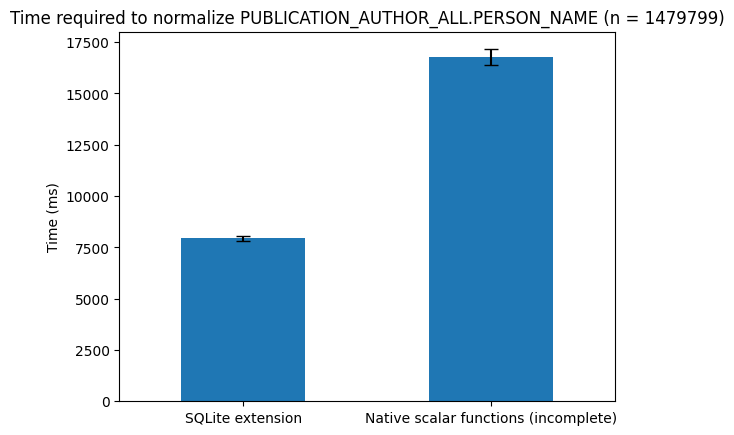
\includegraphics[width=\textwidth]{../img/sqlite_vs_native_scalar_functions.png}
    \centering
    \caption{The performance comparison of the SQLite extension and the composed scalar functions (mean over 10 runs).}
\end{figure}

The Python reference implementation is expectedly much slower than both the SQLite extension and the composed scalar functions.
This is likely caused by the interface read-write overhead of the Python \texttt{sqlite3} library - as compared to the native data access of the SQLite extension.

\textbf{Results assessment}\label{sec:results-assessment}

After the normalization and aggregating the records using the normalized names,
we get \texttt{240001} distinct normalized names in the dataset.

% todo factcheck
The most frequent external author was \textit{B. Abbott} with $1339$ records, followed by $J. Smith$ with $1178$ records.
This raises concerns about the uniqueness of the normalized names - as with $1339$ coauthored publications, \textit{B. Abbott} would be the 99.9 percentile (or the top 7th author),
compared to the internal authors with known identifiers.

\textbf{Issues with the naïve approach}

While the naïve approach is simple and straightforward, it poses several issues.

Firstly, name-based merging can be problematic in the case of the authors with common names, as likely seen in the \hyperref[sec:results-assessment]{results assessment}.

Secondly, there is no support for the existing identifiers from the dataset.
By only inferring the identifier from the name, we willingly discard the existing information about the person.

This could be partially solved by coalescing the inferred identifiers with the existing ones.
Using the SQL \texttt{COALESCE} function, we can create a new column in the \texttt{PUBLICATION\_AUTHOR\_ALL} view that would contain the inferred identifier only if the original one is missing.

However, such approach would only fully work in the case of only internal - or only external authors.
In the case of the internal authors with few records with missing identifiers (e.g. \hyperref[fig:jaroslav-peska]{Jaroslav Peška}),
this would still result in the creation of up to two nodes for the same person (i.e. \texttt{14124313...} for the ``internal'' records and \texttt{jaroslav-peska} for the ``external'' ones).

\begin{mybox}{``On-demand'' naïve identity inference}

To solve the over-merging issue of the authors with common names in the naïve approach, we can slightly modify it.

Instead of merging the records directly in the database, we can merge the records on-demand in the application's visualization layer.
If we e.g. restrict the direct views only to internal authors - and show the external authors only as collaborators of those,
we can reuse the naïve approach quite effectively.

By restricting the domain of the mergeable records to a smaller, tighter subcomunity of the graph (i.e. collaborators of one internal author), 
we can reduce the number of the possible false positives in the merging.

Obviously, this approach still carries the risk of the false positives in case of different external authors with the same name in the same subcommunity.

Also note that this approach only improves the user experience with the application.
Using this, every external author's coauthorship is stored as a separate node in the graph, which can negatively impact the performance of the graph algorithms.
\end{mybox}


\subsection{Distance-based hierarchical clustering}

To solve the issues of the naïve approach, we can try to use the graph structure of the data to infer the missing identities.
One of the possible approaches is to use the \textit{hierarchical clustering} methods to group the nodes with similar attributes together.

In the realm of data mining and statistics, \textit{hierarchical clustering} is an umbrella term for a set of unsupervised learning algorithms for grouping
given data points into a hierarchy of clusters. Typically, these algorithms iteratively merge the closest clusters together, until only one cluster remains.\footnote{In case of top-down clustering, the process is reversed.}
The distance metric used for the clustering can be any metric that defines the similarity between the data points.

In the case of our dataset, we can use the shortest path distance between the nodes in the graph as the distance metric.

We define the merging process as follows:

\begin{enumerate}
    \item Start with a graph with nodes only merged based on explicit identifiers. \texttt{PUBLICATION\_AUTHOR\_ALL} records without an explicit identifier are represented as separate nodes.
    \item Select an arbitrary unmerged node without an identifier.
    \begin{itemize}
        \item Using the \hyperref[sec:naive-approach]{naïve approach}, we find all merge candidates for the selected node. Note that we are using the normalized name equality as the requirement for the merge.
        \item We calculate the distance matrix between the selected node and all the merge candidates.
        \item Using a hierarchical clustering algorithm, we cluster the data points based on the distance matrix. We select the cut-off distance based on the distance distribution.
    \end{itemize}
    \item Go to step 2 until all the non-identifier nodes are merged.
\end{enumerate}


% \newpage

% \subsubsection{Embedding-based clustering}

% Another approach to the problem of inferring the missing identities is to use the \textit{embedding-based clustering} methods.

% The idea behind the embedding-based clustering is to project the nodes of the graph into a lower-dimensional space, where the nodes with similar attributes are close together.

% The graph database Memgraph\footnote{\url{https://memgraph.com/}} offers a built-in implementation of the \textit{node2vec} algorithm\footnote{\url{https://snap.stanford.edu/node2vec/}}.
% We can use this to project the nodes of the graph into a 2D space and then use the clustering algorithms to group the nodes with similar attributes (and same normalized names) together.


% \section{Inferring missing data}

% This section talks about the data inference for missing data. This is a problem mostly for the external authors (with little to no affiliation to CUNI) who can be often only identified by their name and academic titles. We try to come up with a better way of ``filling in the blanks'' - either by using some basic statistics or some data extracted from the social network itself.

% \subsection{Infering identities from the social network}

% Another example is the search for Dmytro Yu Balakin, which yields the following results:

% \begin{itemize}
%     \item Dmytro Yu Balakin
%     \item Dmytro Yu Batakin
%     \item Dmytro Yu. Balakin.
% \end{itemize}

% It is clear that most of those are likely the same person, but the data is not consistent. The first one is the correct one, but the other ones are missing the academic titles and the ``doc.'' prefix. The ``PhD.'' suffix is also inconsistent - sometimes it is ``PhD.'', sometimes ``Ph.D.''. The ``doc.'' prefix is also sometimes missing.

% ...
% ...

% While it might be tempting to solve this "online" by visually merging the entities in the application's visualization layer, this causes multiple issues. The obvious one are the performance implications 

% \section{Analyzing the social network}

% The first contact with the network, description of some basic properties, discovering the features of the data and trying to mine some non-obvious relations from the data.

% \dots
\chapter{Social network boosted search ranking}

Charles Explorer is an academic search engine, which allows the user to search for publications, classes, people and study programmes in the academic domain.

The following sections, we look more into the search engine part of the application, explore the possible issues with the search results ranking, 
and experiment with utilizing the social network data for the search results ranking improvement.

\section{Full-text search}

Full-text search is nowadays an essential part of any information retrieval system. 
Many search engines - including Apache Solr in Charles Explorer - implement the full text search by utilizing the TF-IDF algorithm or similar.
This is a simple and efficient way to rank the search results based on the relevance of the documents to the search query.

The TF-IDF algorithm is based on the term frequency and inverse document frequency of the terms in the documents - a \textit{document} is in general unstructured free text content.
Some entities in our academic search engine map well to this notion of a \textit{document} - e.g. a \texttt{publication} or \texttt{class} both have inherent textual content (titles, abstracts or syllabi).
Unfortunately, this does not hold for all the entities in the system.

As an example, a \texttt{person} entity usually does not have any explicit textual content associated with it. 
When searching for a person interested in a particular topic, the search engine has to rely on the textual content of the publications, classes, 
or other entities associated with the person, i.e. traverse - at least implicitly - the knowledge graph (or the social network of the person).

A simple solution to this problem would be to represent every person as a document, concatenating all the textual content of the entities associated with the person.
This can be further refined by assigning different weights - e.g. to the different types of entities (a \texttt{class} might be more important than a \texttt{publication}), 
or different concatenated parts of the documents (e.g. the publication title and class name are more important than the abstracts and syllabi).

Regarding adding new entities related to a given person, the concatenation also serves us well - we simply append the new entity's content to the person's document and reindex it.

However, this approach also has several drawbacks. First of all, assuming we're building a general academic search engine allowing for search in publications, classes and people, we would be indexing the same content multiple times.
This is not only inefficient in terms of storage, but also prone to update errors - there is multiple copies of the same content, which have to be updated separately.
The second issue arises from the concatenation - if any of the person's associated entities changes, the whole document has to be reindexed.
However, this might be less of a problem than the first issue, as it's not too common for academic records to get updated or removed - at least in comparison to the number of new records being added.

\subsection{Result ranking in the naive case} \label{search-ranking-issues}

Result ranking in information retrieval refers to the ordering of the search results when presented to the end user. This is often based on the relevance of the documents to the current search query.
The relevance-based ranking is often enough for the basic use case - the user is presented with the most relevant documents first, and can further explore the less relevant ones if needed.

While it might seem a bit superficial, the ranking is in fact still part of the information retrieval process. 
%% todo make into citations
As multiple studies show \footnote{https://link.springer.com/article/10.1007/s11151-014-9435-y}\footnote{https://link.springer.com/article/10.1007/s10791-010-9150-8}, 
the ranking of the search results positively correlates with the click-through rate of the results 
- likely because of the typical top-left to bottom-right reading pattern of the users.
This can be further affected by other, more technical factors - such as the need for an additional user action like scroll or pagination to see the results further down the list.

%% https://link.springer.com/article/10.1007/s10791-010-9150-8 - Re-ranking search results using an additional retrieved list

Considering a simple tf-idf based search engine, the ranking of the search results is based on the relevance of the documents to the search query.
This is directly related to the term frequency of the query in the document - for a fixed query and document collection, we can forget about the inverse document frequency, as it's constant over all the documents.
Ranking the documents solely based on the term frequency might however lead to unfavourable results - especially in the case of a proxy-representation of a given entity.


\begin{figure}[ht!]
    \captionsetup{width=.9\linewidth}
    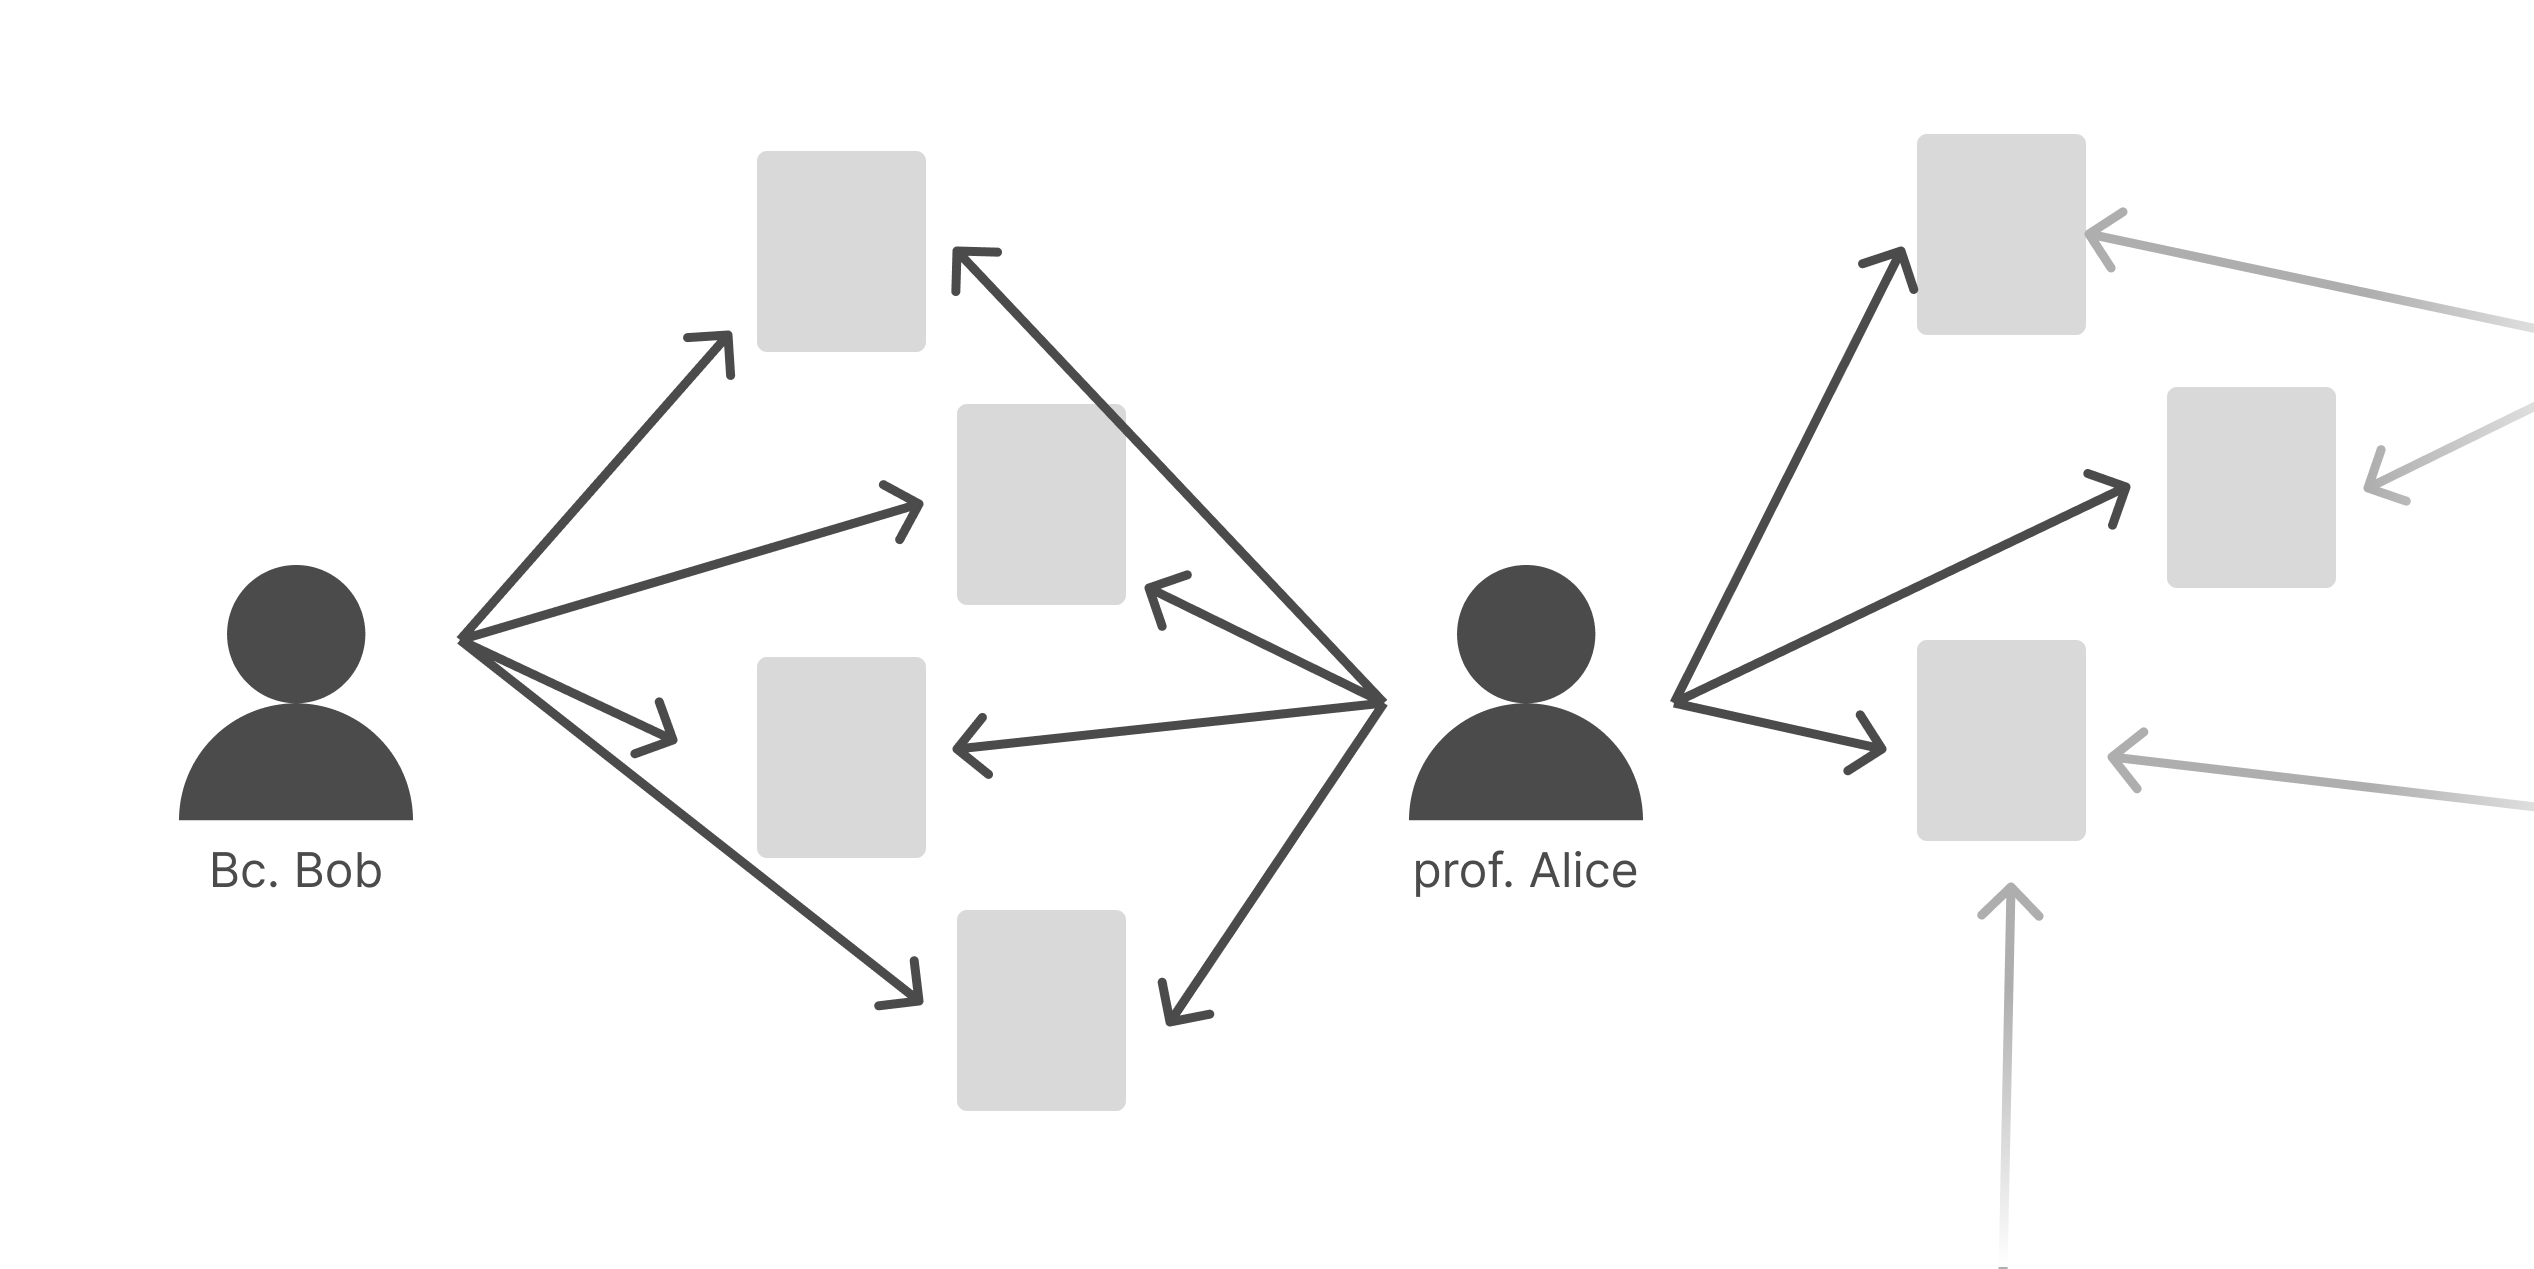
\includegraphics[width=0.8\textwidth]{../img/bob-alice-soc-netw.png}
    \centering
    \caption{Simple representation of the social network of Alice and Bob.}
\end{figure}

Let us explore the issues on an example where we represent people as documents, concatenating the textual content of the entities associated with them.
Consider two academic researchers in our system - \textit{prof. Alice} and \textit{Bc. Bob}. 
Bob is a student of Alice, and has published several papers on \textit{Information retrieval} with her. Aside from those, Bob has not published any other papers.
On the other hand, Alice has published a lot of papers on various topics - related to IR, but also to other similar fields. 
See a simple representation of their social network above.

Note that aside from the common publications, Bob has no other entities associated with him, while Alice has other publications with other co-authors.

\begin{figure}[ht!]
    \captionsetup{width=.9\linewidth}
    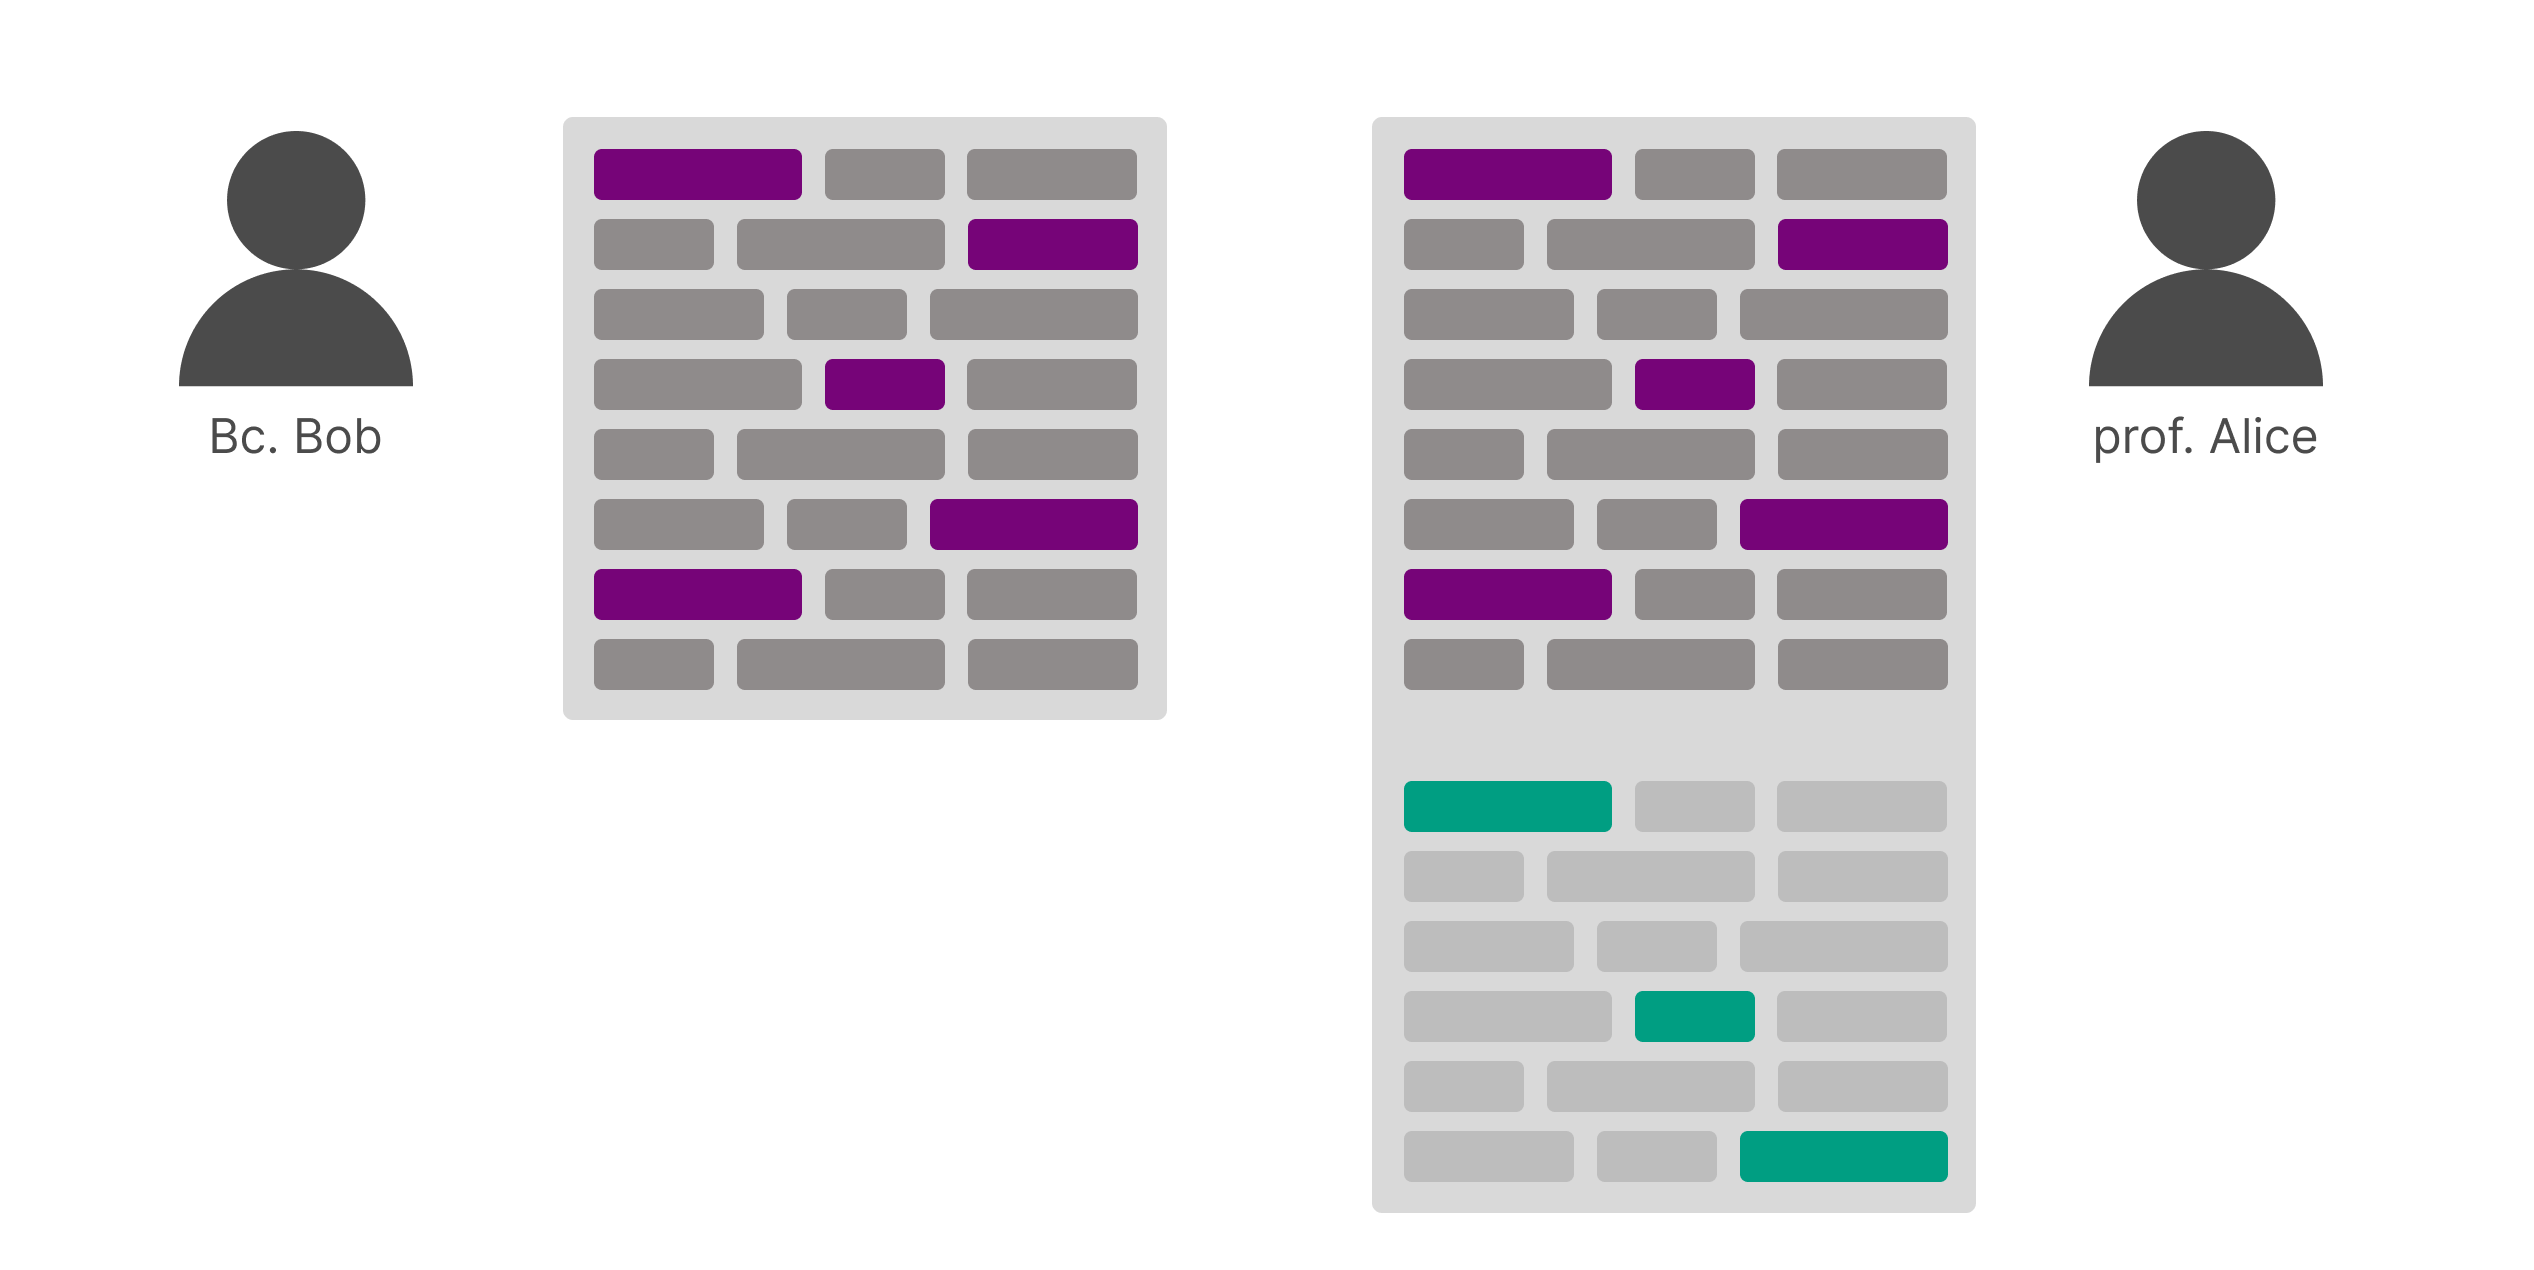
\includegraphics[width=0.8\textwidth]{../img/bob-alice-representations.png}
    \centering
    \caption{Concatenating representations of Alice and Bob as documents.}
\end{figure}

We see that the document of Bob is shorter than the one of Alice, because he has less associated entities. We also notice that the Alice's document fully contains the Bob's document.
    
The colored terms represent the current search query - if Alice only published papers on the topic of the query with Bob, the term frequency of the 
query in Bob's document would be strictly higher, because of the shorter document length.
In case Alice also publishes on the topic with other co-authors, it gets harder to reason about which of the term frequencies is higher.

The relation between the tf-idf scores of the documents of Alice and Bob is expressed as follows:
\begin{subequations}
\begin{align}
\text{tf}(q, d_{\text{Bob}}) \times \text{idf}(q, D) &\stackrel{?}{>} \text{tf}(q, d_{\text{Alice}}) \times \text{idf}(q, D) \\
\text{tf}(q, d_{\text{Bob}}) &\stackrel{?}{>} \text{tf}(q, d_{\text{Alice}})
\end{align}
\end{subequations}

Normalized term frequency $\text{tf}_{q,d}$ of a term $q$ in a document $d$ is defined as the number of times the term $q$ appears in the document $d$ (denoted by $f_{q,d}$),
divided by the total number of terms in the document $d$ (the document's length).

\begin{subequations}
\begin{align}
\frac{f_{q, d_{\text{Bob}}}}{\text{len}(d_{\text{Bob}})} &\stackrel{?}{>} \frac{f_{q, d_{\text{Alice}}}}{\text{len}(d_{\text{Alice}})} \Biggm/ \;^{-1} \\
\frac{\text{len}(d_{\text{Bob}})}{f_{q, d_{\text{Bob}}}} &\stackrel{?}{<} \frac{\text{len}(d_{\text{Alice}})}{f_{q, d_{\text{Alice}}}} \Biggm/ \textit{assuming that } \mathit{f_{q, d_{\text{Bob}}} = f_{q, d_{\text{Alice}}}} \label{eq:51assumption}\\
\text{len}(d_{\text{Bob}}) \;&<\;\text{len}(d_{\text{Alice}})
\end{align}
\end{subequations}

Since we have assumed that Alice's document is a superset of Bob's document, the result inequality holds - and therefore the tf-idf score of Bob's document is higher than the one of Alice's document.

Note that the assumption in the equation \ref{eq:51assumption} is only true for the cases when Alice does not publish any other papers on the topic of the query with other co-authors.

% Because of this, the document representation of Bob will be short, compared to the one of Alice.
% Assuming the search query is \textit{Information Retrieval} - and there are no other publications or classes related to this topic in the system - 
% the search engine will consider Bob as the more relevant person for this topic. This is becuase the term frequency of the query in Bob's document is higher than in Alice's document - solely because of the length.

In either way, this approach most likely will not provide the desired outcome - while Bob has published papers only on the given topic - and therefore has higher tf-idf relevance to the query,
it is likely that Alice is the more relevant person for the searching user, since she is more experienced in the topic.

\section{Re-ranking}

In the following sections, we go over different existing re-ranking strategies utilized in other systems and explore the possibilities of using the social network data for the re-ranking in Charles Explorer.

\subsection{Existing re-ranking strategies}

In the current (2024) commercial search engines, there are often multiple re-ranking strategies available to the users.
Unfortunately, only a small portion of the engines actually discloses the details of the re-ranking algorithms used - perhaps to protect the intellectual property and the competitive advantage.

The common grounds for all those systems is the two-stage search pipeline - in the first stage, a traditional search engine is used to retrieve the initial set of results.
Then, these results are re-ranked using a different algorithm. 

While it might seem redundant, this approach allows the second algorithm to focus only the more relevant results, and be perhaps more computationally expensive.
Unfortunately, this also means that the re-ranking algorithm is not able to affect the initial search results - it can only change the order of the results.
It also brings in the issue of pagination - if the user has to go through multiple pages of the search results, the re-ranking might not be as effective,
as it only affects the current page of the results.

The re-ranking algorithms can be based on various factors - the user's previous interactions with the system, total popularity (click-through rate) of the items,
diversity of the results %link to the MMR papers https://www.google.com/search?client=firefox-b-lm&q=Maximal+Marginal+Relevance 
or NLP analysis of the documents. Especially the last one seems to be gaining traction in the recent years, as the applications of LLM models are becoming more widespread.

\subsection{Graph data-based reranking}\label{graph-based-reranking}

As we discussed in \ref{search-ranking-issues}
, the traditional tf-idf based search engine might give unsatisfactory results in the case 
of a proxy-representation of a given entity.
We might try to address this issue by utilizing the social network data for the re-ranking of the search results.

As mentioned in the previous subsection, many commercial search engines use a two-step search pipeline - the first step retrieves the initial set of results,
and the second step re-ranks them using a different algorithm. This sounds like a good fit for our problem - we use the traditional tf-idf based search engine 
to retrieve the initial set of results, and then re-rank them using the social network data. 

Only using the graph data for the search has several drawback described in the next section (\ref{graph-based-search}).

When it comes to reranking the existing search results, we utilize the social network data in several ways.

\begin{itemize}
    \item \textbf{Global node statistics}: As illustrated on the example of Alice and Bob above, 
    we can use the global statistics for the nodes in the social network to re-rank the search results. 
    These include - but are not limited to - the node degree (number of connections), centrality measures, or the number of common neighbours.

    Such statistics can be precomputed for every node in the social network before the search and stay constant over all the search queries.

    \item \textbf{Query relevant node statistics}: Unlike the global node statistics, query-relevant node statisics are computed only for the nodes in the search results.
    
    These can perhaps define the node's relevance better (e.g. the number of query-relevant publications connected to a given person), but are often more computationally expensive to compute.
    Given the variability of the queries, it is also harder (or impossible) to precompute these statistics.
\end{itemize}

%% todo structure
\subsection{Graph data-based search} \label{graph-based-search}

It would also be possible to use the social network data to entirely replace the concatenated person representations in the search engine - we could 
only search through the ``first-order entities'' (i.e. classes and publications) and then query the social network graph for the people associated 
with the results of the search. 

This approach has several drawbacks - aside from the questionable performance and scalability / developer effort, it also might not be as effective as the concatenated representation.

With the concatenated approach, we have to retrieve only \textasciitilde{} 30 results (people) for every page of the search results. 
Those are also already ranked by the relevance to the query - even though this might not be perfect, the tf-idf based ranking is still a good approximation.

With the proposed graph-based approach, we would have to retrieve many more publications and classes on each search - note that we are no longer 
looking for the most-relevant class or publication, but for the most-relevant person - which is rather an aggregation of the relevance of the associated entities.
This might lead to a lot of unnecessary data retrieval and processing and become the bottleneck for the possible applications built on such data.


\section{Assessing reranking performance}

To determine the performance of our proposed re-ranking solution, we establish benchmarks to compare the results of the traditional tf-idf based search engine with the social network enhanced search engine.

Even though we have only talked about person entities in the previous sections, we will conduct the benchmarking on the ranking of the search results for \textbf{publication} records.
This is because the publications are uniquely identifiable (unlike people - see \ref{sec:inferring-missing-identities} for more details) 
and they have implicit textual content associated with them - the title, abstract and keywords.
Note that the issues from \ref{search-ranking-issues} still apply for the publications - \cite{aseo} mention different approaches to \ac{ASEO}.
By overusing certain keywords in the publication titles and abstracts, the authors can artificially increase the relevance of their publications to the search queries.

\subsection{Benchmarking the search results ranking}

The common denominator for many of the ranking measures - like discounted cumulative gain or mean reciprocal rank - is the \textit{user interaction}.
The user is presented with the search results and picks the most relevant one or scores the results based on the relevance to the query.

Unfortunately, this is not applicable to our case - while we are tracking the user interactions in the Charles Explorer web appplication, the amount of collected data is far too low to be statistically significant.

\begin{mybox}{}
    The following section is described in greater detail in my blog posts series \textit{Benchmarking Charles Explorer search result rankings}\footnote{\url{https://jindrich.bar/edu/thesis-blog/}}.
    
    The blog posts contain the detailed description of the process of collecting the search queries for the benchmarking of the search results ranking in Charles Explorer.

    Since the blog posts are rendered Jupyter notebooks, they also contain the code snippets used for the data collection and analysis.
    The implementation of all the steps - i.e. data collection, data preprocessing, and the benchmarking itself - is fully reproducible and available in the embedded code snippets.
\end{mybox}

To establish a gold standard for the search results relevance, we do not have to rely solely on human interactions.

Elsevier Scopus\footnote{https://www.elsevier.com/products/scopus} is a large academic database, which provides a search engine for the academic publications.
Aside from the web application, it also provides a REST API for consuming the data programmatically.

We use the Scopus API to retrieve ranked lists of publications for a given query, and then use the ranking of the publications as the source of the ``global relevance'' for the search query in the benchmark.
Simply put, by comparing the (ranking of the) search results in our search engine to the results of the Scopus search engine, we determine the relevance of the search results.

We are expecting the search results of the Scopus search engine to be more precise and relevant than the ones of the Charles Explorer search engine -
Scopus is a commercial product with a large team of developers and researchers, while Charles Explorer is a small academic project.
The data available to scopus also contain details about the citations of the publications and author profiles, which can be used to further improve the search results ranking.

\subsection{Sampling the search query set}

As the first step, we need to sample the \textit{search query set} for the benchmark. 
Since we want to rule out possible biases - or at least mitigate their impact - we need a large and diverse enough set of queries to compare the search engines on.

Generating these manually would be time-consuming and error-prone. 
Therefore, to solve this issue, we use a \textit{wordnet} - a lexical language database of English.
We use it to generate a large set of diverse queries, perhaps less biased than a manually generated set.

We start by selecting a set of \textit{seed words} - in our experimental case, those were the words \textit{``field of study''} and \textit{``medicine''}.
Then, we traverse the wordnet to recursively find the hyponyms of those seed words, up to a certain depth.

Running this process for the seed words \textit{``field of study''} and \textit{``medicine''} with the depth of 4, we get a set of \texttt{915} search queries.

While this approach gives us a sizable set of queries, we have no guarantee of the quality of the queries - they might be too general or too specific, or not relevant to the academic domain at all.
One of our goals was also to ensure the fairness of the query set - this is not guaranteed by the wordnet traversal either, as the queries might be too similar to each other (or target the similar topics in the publications).

\subsubsection{Ensuring the query set fairness}

While \textit{fairness} is a largely subjective measure, we let the available data guide us in this case.
For the \textit{academic publications}, we have their \textit{titles}, \textit{abstracts}, \textit{keywords}, \textit{faculty affiliations} and \textit{authors} avaialble in our system.

Since titles, abstracts and keywords are free text fields, we omit them from our analysis - the preprocessing of the text data is a complex task on its own.
Given the nature of our experiment - i.e. measuring the impact of using the social network data for the search results ranking - we have to leave the authorship information out as well.

This process leaves us with the faculty affiliations.

Charles University has \textit{17} faculties, each with a different focus and research areas.
Each publication in our data is attributed to exactly one faculty.
This allows us to use the faculty affiliations as a proxy for the fairness of the search queries.

\textbf{Kullback-Leibler divergence}

As the fairness measure, we compare the distribution of the faculty affiliations in the search query results 
to the distribution of the faculty affiliations of all the publications in the system.

The standard way of comparing probability distributions is the \textit{Kullback-Leibler divergence} - a measure of how one probability distribution diverges from a second, expected probability distribution.

For discrete probability distributions $P$ and $Q$ defined on the same sample space $\Omega$, the Kullback-Leibler divergence from $Q$ to $P$ is defined as

$$
D_{KL}(P||Q) = \sum_{\omega \in \Omega} P(\omega) \log \frac{P(\omega)}{Q(\omega)}
$$

The KL-divergence is always non-negative, and is zero if and only if $P$ and $Q$ are the same distribution.

With the measure of the fairness of the search query set established, we now proceed to the benchmarking of the search results ranking in Charles Explorer.

By sampling up to 30 results for each search query from the Charles Explorer search engine, we acquire the faculty distribution for the entire search query set ($N = 915$).
We then compare this distribution to the distribution of the faculty affiliations of all the publications in the system.

\begin{figure}[ht!]
    \captionsetup{width=.9\linewidth}
    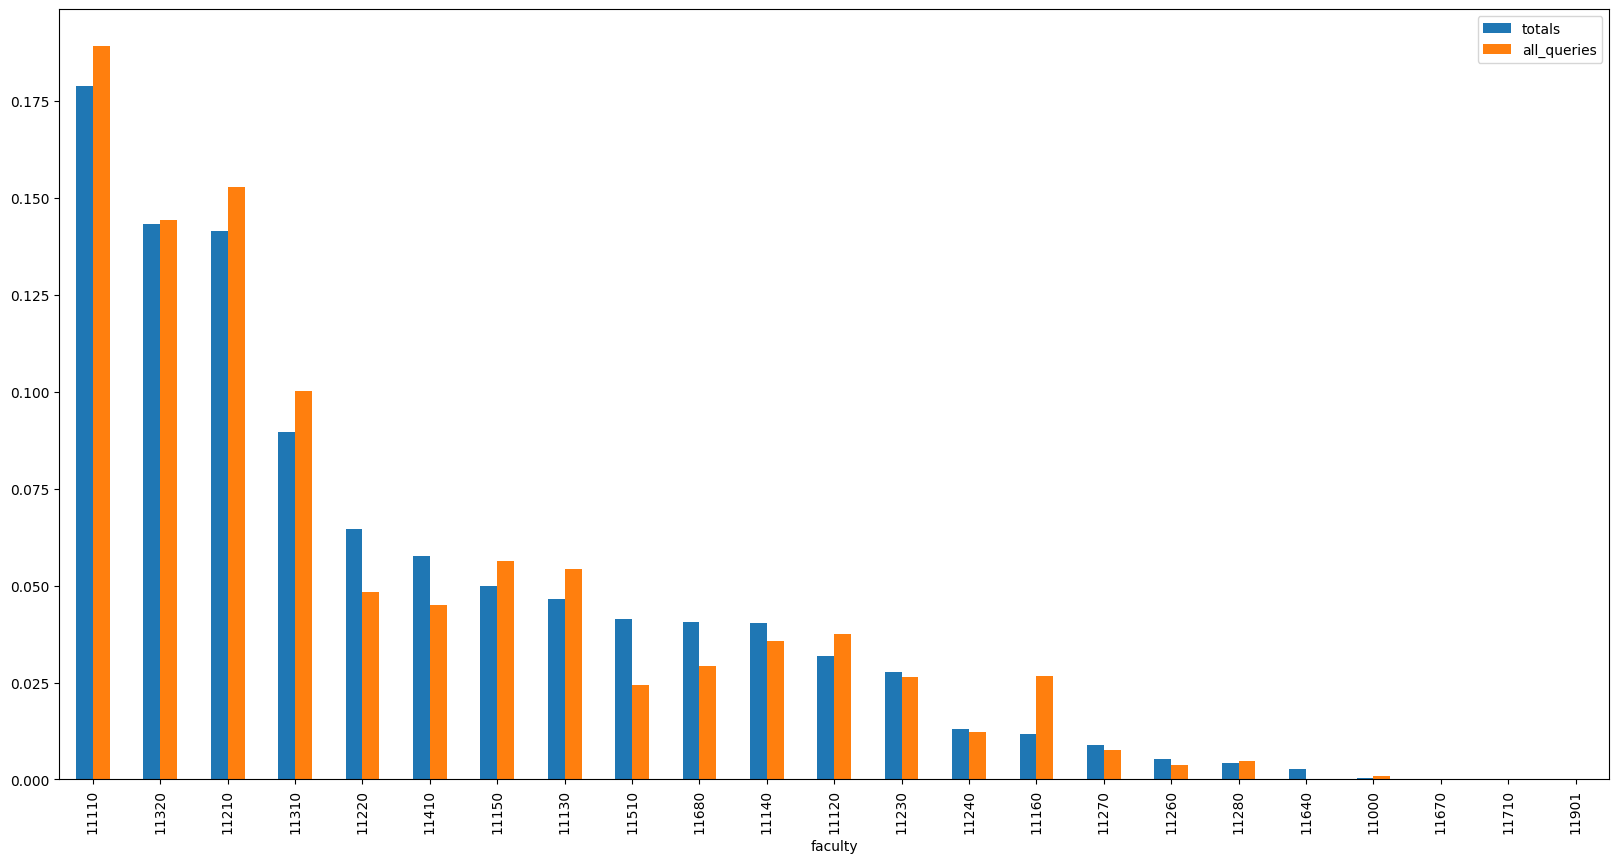
\includegraphics[width=0.8\textwidth]{../img/all-queries-vs-totals.png}
    \centering
    \caption{Comparing the faculty distribution of the search query results \textit{(orange, right)} to the distribution of all the publications in the system \textit{(blue, left)}.}
\end{figure}

The Kullback-Leibler divergence of the faculty distribution of the \textbf{search query results} from the distribution of \textbf{all the publications} in the system is approximately \texttt{0.0471}.

\textbf{Optimizing the KL-divergence}

With the defined measure of the fairness of the search query set, we now try to optimize it.
In our case, optimizing the KL-divergence means \textit{finding a subset} of search queries which would minimize the divergence of the faculty distribution of the search query results from the distribution of all the publications in the system.

Unfortunately, this poses serious challenges. 
Finding a subset with an optimal aggregate property is a well-known NP-hard problem - often referred to as the \textit{0-1 knapsack problem} or the \textit{subset sum problem}.
Even worse, we cannot simply reuse some of the existing algorithms for these problems, as those rely on the distributivity and associativity of the sum operation. 
This is however not the case for the KL divergence.

Similarly to the sum of the item values (in the Knapsack problem), the KL divergence is evaluated on the entire set, but unlike the sum, the items themselves do not have any “value” - and their contribution to the KL divergence changes depending on the other items in the set. 
This leaves us with a limited choice of algorithms to solve the problem. 
Because of the complexity of the problem and its smallish role in this work, we use a simple random search. 

This approach works in two steps:

%% todo pseudocode algorithm for the optimization
\begin{enumerate}
    \item Repeatedly sample a random subset of size $k$ of the search queries, keeping track of the subset with the lowest KL divergence.
After a fixed number of iterations, take the subset with the lowest KL divergence.
    \item From the $k$-sized subset, repeatedly remove the search query with the highest contribution to the divergence.
Stop when the KL-divergence stops decreasing, i.e. we cannot remove any more search queries to decrease the divergence, or we've reached the minimum subset size $l$.
\end{enumerate}

This is a simple and computationally cheap approach, but it might not always find the optimal solution.
Furthermore, since the KL-divergence is a non-convex function, the second step of the algorithm might get stuck in a suboptimal solution.
While this could be mitigated using a more complex optimization algorithm (e.g. simulated annealing etc.), experimental results show that the simple random search is sufficient for our purposes.

\begin{figure}[ht!]
    \captionsetup{width=.9\linewidth}
    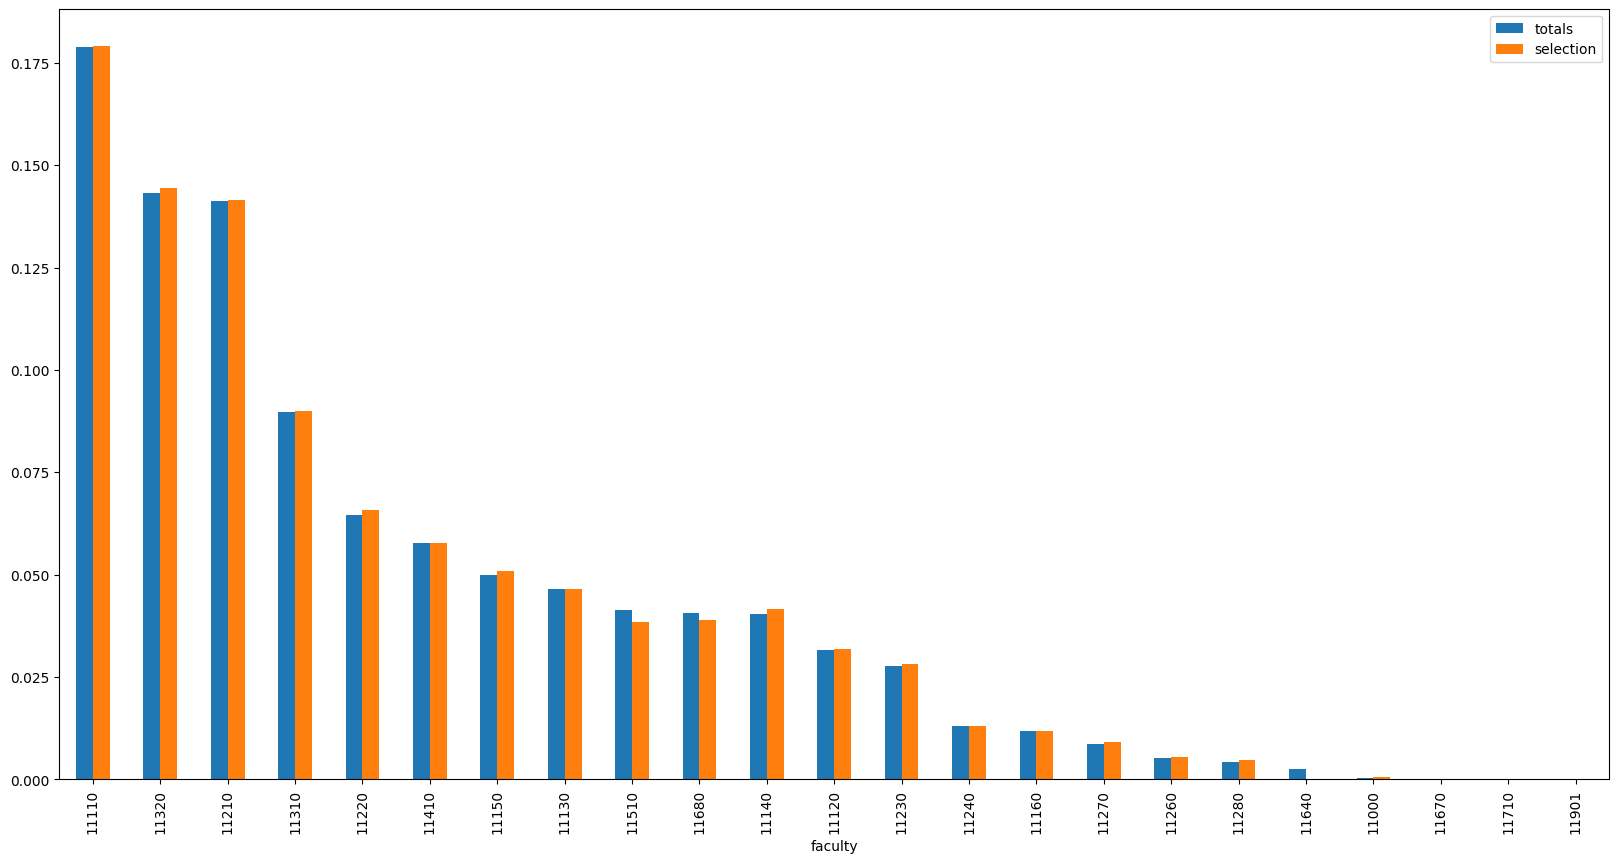
\includegraphics[width=0.8\textwidth]{../img/all-queries-vs-totals-corrected.png}
    \centering
    \caption{Comparing the faculty distribution of the search query results \textit{(orange, right)} to the distribution of all the publications in the system \textit{(blue, left)} \textit{after running the optimization algorithm}.}
\end{figure}

Running the optimization algorithm with $n = 10000$ initial random samples of size $k = 300$ on the search query set, we arrive at a set of $174$ queries with the search result KL-divergence of \texttt{0.00317}. 
This is a significant improvement over the original divergence of \texttt{0.0471} and we will consider this a fairer subset of the search queries for the benchmarking.

\subsection{Collecting the data}

Since our proposed benchmark only evaluates the search results ranking, we collect the search results for the benchmark queries in advance.
Similarly, we also collect the data from the Scopus API for the same queries, as the automated relevance feedback.

While collecting the search results from the Charles Explorer search engine is straightforward since the API is available to us, 
the Scopus Advanced search feature requires us to use a special query language\footnote{\url{https://schema.elsevier.com/dtds/document/bkapi/search/SCOPUSSearchTips.htm}} to submit the search queries. 
This query language offers a set of Prolog-like functors, 
each related to a specific field - or a set of fields - of the publication record. 
The attributes of these functors are used in a \textit{substring search} on the specified fields.

Apart from this, the query language also supports logical operators, such as \texttt{AND}, \texttt{OR}, and \texttt{AND NOT}.

We will use two of the available functors: \texttt{TITLE-ABS-KEY} and \texttt{AF-ID}:

\begin{itemize}
    \item \texttt{TITLE-ABS-KEY} searches for the specified substring in the title, abstract, and keywords of the publication record. 
    In this regard, it is similar to the full-text search in Charles Explorer, which searches in the same fields.
    \item \texttt{AF-ID} filters the search results by the organisation affiliation of the publication. This is useful for filtering the search results to only those publications where at least one of the authors is affiliated with Charles University. Since Elsevier Scopus contains many records not affiliated with Charles University (but Charles Explorer only contains such records), this will help us to get a more comparable sets of search results.
\end{itemize}

By calling the Scopus API, we get the search results in JSON format, which we then process and store in our database for the benchmarking.

\begin{figure}[ht!]
        \scriptsize
        \centering
        \begin{tabular}{|l|l|l|l|l|l|l|}
        \hline
            ~ & ranking & totalAuthors & scopusId & pubYear & citationCount & referenceCount \\ \hline
            ranking & 1.000000 & 0.038005 & 0.081229 & 0.109848 & 0.062467 & 0.053487 \\ \hline
            totalAuthors & 0.038005 & 1.000000 & 0.033948 & 0.040538 & 0.113336 & 0.094358 \\ \hline
            scopusId & 0.081229 & 0.033948 & 1.000000 & 0.806411 & 0.015393 & 0.243830 \\ \hline
            pubYear & 0.109848 & 0.040538 & 0.806411 & 1.000000 & 0.033019 & 0.283521 \\ \hline
            citationCount & 0.062467 & 0.113336 & 0.015393 & 0.033019 & 1.000000 & 0.218415 \\ \hline
            referenceCount & 0.053487 & 0.094358 & 0.243830 & 0.283521 & 0.218415 & 1.000000 \\ \hline
        \end{tabular}
    \caption{Correlation matrix of the Elsevier Scopus search results numeric attributes.} 
\end{figure}

We see that the \texttt{ranking} column - the position of a publication in the search results - is only very weakly correlated with the other numeric attributes of the search results.
This suggests that the default Scopus ranking is mostly influenced by the full-text search and does not take much reranking into account.

It also suggest that the Scopus result ranking might not be too dependent on the social network measures and that we might not be able to improve the ranking 
by using the social network data (as the ``explicit'' social network data like the citation count or the reference count are not correlated with the ranking).

\subsection{Simulating relevance feedback}

With the data collected, we now proceed with the actual analysis of the search results ranking in Charles Explorer.

Considering the Scopus search results as the gold standard, we calculate the per-query precision, recall and $F_1$ score for the search results of Charles Explorer.

\begin{figure}[!ht]
    \captionsetup{width=.9\linewidth}
    \centering
    \begin{tabular}{|l|l|l|l|}
    \hline
        \textbf{Query} & \textbf{Precision} & \textbf{Recall} & \textbf{$F_1$ score} \\ \hline
        physics & 0.043011 & 0.040000 & 0.041451 \\ \hline
        bolus & 0.125000 & 0.121212 & 0.123077 \\ \hline
        draft & 0.010870 & 0.010753 & 0.010811 \\ \hline
        $\hdots$ & $\hdots$ & $\hdots$ & $\hdots$ \\ \hline
    \end{tabular}
    \caption{Per-query precision, recall and $F_1$ score for the search results of Charles Explorer.}
\end{figure}

After aggregation over all the queries, this gives us the following unfavourable statistics:

\begin{figure}[!ht]
    \captionsetup{width=.9\linewidth}
    \centering
    \begin{tabular}{|l|l|}
    \hline
        Mean & 0.208727 \\ \hline
        Standard deviation & 0.211699 \\ \hline
        Minimum & 0.010101 \\ \hline
        25\% & 0.074786 \\ \hline
        50\% & 0.137028 \\ \hline
        75\% & 0.265263 \\ \hline
        Maximum & 1.000000 \\ \hline
    \end{tabular}
    \caption{Aggregated statistics of the $F_1$ score for the search results of Charles Explorer.}
\end{figure}

We see that the current Charles Explorer search results differ quite a lot from the Scopus search results. 
This can be caused by mutiple reasons - either the publications are not present in the Scopus database, or the queries are not specific enough - and the search results are returning partially disjoint sets of publications.

Note that this is an issue that goes beyond re-ranking the Charles Explorer search results. 
We cannot quantify the benefit of reordering the search results if we consider all the search results irrelevant.
This hinders our ability to use the Scopus search results ranking as the proxy for the relevance feedback.

Since this thesis is focused on the search result ranking algorithms, we will proceed with the benchmarking as planned. 
However, to improve the relevance score assignment, we add a \textit{similarity search} step. 
 
In the $F_1$ score calculation, we are only matching the Charles Explorer search results with the Scopus search results by the publication title (case-insensitive). 
This matching criterion is prone to even the slightest variations in the publication titles, which can lead to false negatives.

\subsubsection{Inferring the publication relevance with semantic search}\label{semantic-search}

In the proposed \textit{similarity search} step, we use the similarity of LLM (Large Language Model) embeddings to match the publication titles. 
This should help us to relate the publications missing from the Scopus search results to the ones present there and assign them a relevance score.

\begin{mybox}{LLM embeddings}

    \textit{LLM embeddings} are vector representations of a given text, generated by a large language model.
    While those can be arbitrary vectors, embeddings are usually optimized to capture the semantic meaning of the text. 
    
    This means that texts with similar meanings should have similar embeddings - i.e. the (cosine) similarity of the embedding vectors should be high.
\end{mybox}

We enhance the relevance calculation with the similarity search process as follows:

\begin{enumerate}
    \item By the means of an \textit{LLM embedding model}, we precalculate the embeddings for the publication titles of the Elsevier Scopus search results. 
    We store these embeddings in a vector database.
    \item For each publication title in the Charles Explorer search results, we calculate its embedding. 
    In the database, we search for the nearest embedding among Scopus search results embeddings. 
    Futhermore, we require the retrieved document to be a result of the same query (in Elsevier Scopus) as the Charles Explorer search result.
    \item We calculate Charles Explorer document’s inferred relevance from the most similar document’s attributes - e.g. its position in Scopus search.
\end{enumerate}

For the document embedding, we use the \texttt{all-MiniLM-L6-v2}\footnote{\url{https://www.sbert.net/docs/sentence_transformer/pretrained_models.html}} sentence - transformer model. 
This is a general-purpose English embedding language model designed for running on consumer-grade hardware. 
Due to its small size and competitive performance, it’s often used for the real-time use-cases, like semantic search or RAG (Retrieval-Augmented Generation).

For the similarity search on the embeddings we use the ChromaDB database\footnote{\url{https://www.trychroma.com/}}. 
ChromaDB is a vector database designed for the similarity search on the embeddings, with support
for enhancing the search results with the additional metadata attributes of the documents.

\newpage

\begin{figure}[ht!]
    \captionsetup{width=.9\linewidth}
    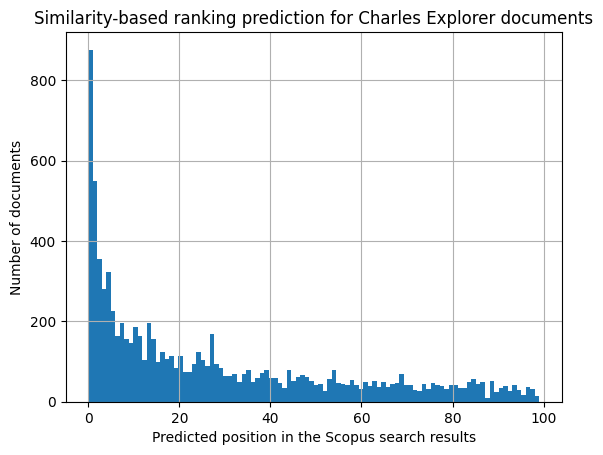
\includegraphics[width=0.8\textwidth]{../img/llm-embedding-positions-hist.png}
    \centering
    \caption{Histogram of inferred positions of the Charles Explorer search results in the Scopus search results.}
\end{figure}

This process gives us the predicted rankings which follow a rather skewed distribution. 
However, this does not pose a serious problem to our benchmark.

Firstly, we are not trying to predict the exact ranking of the search results, but rather to assign a relevance score to each search result. 
The peak of the distribution is at the top of the rankings, 
which is in line with the well known tendency of human users 
to have much clearer opinion about the few top results than the long tail of the search results (as described by e.g. \cite{9357332}).

Secondly, the left-skewed distribution might be caused by non-uniform lengths of the search result lists. 
Since for some of the queries, Scopus returns only a few relevant search results (100 is only the maximum limit), 
the resulting predicted rankings will be skewed towards the top of the list for these queries.

\subsection{Calculating the base nDCG}

Using the original ranking positions and the predicted ranking positions as the source for the 
relevance feedback, we calculate the \textit{nDCG} (Normalized Discounted Cumulative Gain) score for the 
search result ranking.

DCG score for a single search result list is calculated as the sum of the relevance scores of the search results, discounted by their position in the ranking.

$$
DCG_\text{list} = \sum_{i=1}^{N} \frac{2^{rel_i} - 1}{\log_2(i + 1)}
$$

The IDCG score is the DCG score of the ideal ranking of the search results, i.e. the items in the list are sorted in descending order by $rel_i$.

Normalized DCG score is then calculated as the ratio of the DCG score to the IDCG score.

$$
nDCG_{\text{list}} = \frac{DCG_\text{list}}{IDCG_\text{list}}
$$

To transform the predicted Scopus rankings from \ref{semantic-search} into relevance feedback, 
we introduce a new function $rel_q(d)$.

For a given query $q$, the document $d$ is considered to have relevance of $rel_q(d)$, 
which is \textit{inversely proportional} to its predicted ranking. 
This is necessary for the \textit{nDCG} score calculation, which requires more relevant documents 
to have higher relevance scores.

The inverse proportionality is achieved by the following formula:
\[rel_q(d) = \frac{a}{\text{rank}_q(d) + 1}\]

where $a$ is a constant that scales the relevance scores and can help achieve better 
stability of the nDCG score with respect to rounding errors.

For the purpose of the experiments in this thesis, we set $a = 5$. 
The $+1$ in the denominator is necessary to avoid division by zero, as our rankings are $0-$based.

While it would be possible to achieve the ranking $\rightarrow$ relevance transformation via e.g. subtracting the predicted ranking from the total number of search results, 
our proposed method with $rel_q(d)$ introduces a \textit{non-linear} transformation of the predicted rankings. 
This differentiates better between the search results that are ranked higher in the Scopus search results. 
This is again in line with the beforementioned tendency of the human users to have clearer opinions about the top search results.

nDCG calculation over the search results of Charles Explorer with the predicted relevance scores from \ref{semantic-search} gives us the following results:

\begin{figure}[!ht]
    \captionsetup{width=.9\linewidth}
    \centering
    \begin{tabular}{|l|l|l|l|}
    \hline
        ~ & dcg & idcg & ndcg \\ \hline
        mean & 14.919819 & 19.167405 & 0.761607 \\ \hline
        std & 16.810894 & 17.665142 & 0.180979 \\ \hline
        min & 0.094340 & 0.094340 & 0.405669 \\ \hline
        25\% & 5.250473 & 7.704989 & 0.627563 \\ \hline
        50\% & 9.527864 & 14.840570 & 0.736246 \\ \hline
        75\% & 18.064385 & 24.112511 & 0.934206 \\ \hline
        max & 104.693354 & 104.693354 & 1.000000 \\ \hline
    \end{tabular}
    \caption{Aggregated statistics of the nDCG score for the original search results of Charles Explorer (\textit{query count = $149$}).}
\end{figure}

The mean nDCG score of $0.761607$ suggests that the search result ranking in Charles Explorer already works well - and that the relevance feedback based on the predicted Scopus rankings gives us a good approximation of the relevance of the search results.

\subsection{Using graph metrics for re-ranking}

With the relevance feedback and baseline benchmark values established, we can now proceed with the re-ranking of the search results in Charles Explorer using the social network data.

Due to the large size of the social network %%( todo number of nodes + edges)
we prefer to use local graph statictics - or \textit{query relevant} statistics, as defined in \ref{graph-based-reranking}.

\subsubsection{Ego betweenness centrality}\label{ego-betweenness}

The “betweenness centrality” is a graph node measure that quantifies the importance of a node in a graph. 
It is calculated as the number of shortest paths between all pairs of nodes that pass through the node in question:

\[g(v) = \sum_{s \neq v \neq t} \frac{\sigma_{st}(v)}{\sigma_{st}}\]

where $s$, $t$ and $v$ are nodes in the graph, $\sigma_{st}$ is the number of shortest paths between nodes $s$ and $t$, and $\sigma_{st}(v)$ is the number of shortest paths between $s$ and $t$ that pass through $v$.

While this is usually calculated in the context of the entire graph, it is an useful measure for ego-networks too, as it can help us quantify the importance of a node in its local neighbourhood. 
\cite{egonetworkbetweenness} have shown that for real-life networks, the ego betweenness centrality often correlates with the actual global betweenness of a node in the graph.

In our data, the collaboration graph is bipartite - the nodes are either publications or people and there are no edges between the nodes of the same type.
This means that the ego betweenness centrality of a publication is in fact proportional to the number of people that have collaborated on the publication.

\subsubsection{2-hop betweenness centrality}
Similar to the \ref{ego-betweenness}, we calculate the 2-hop betweenness centrality as the betweenness centrality of a node 
in a subgraph induced by the node and its 2-hop neighbourhood.

In our case of the bipartite collaboration graph, the 2-hop betweenness centrality of a publication is no longer proportional only to the number of people that have collaborated on the publication,
but also to the number of other publications that the people have collaborated on.

Note that this concept can be further extended to the $k$-hop betweenness centrality, but the computational complexity of the centrality calculation grows exponentially with the $k$.
Materializing the induced subgraphs for the $k$-hop betweenness centrality calculation also poses a challenge in regard to the memory consumption. 

In our experiements, we only use the $1-$ and $2-hop$ betweenness centrality as the query-relevant node statistics.
\chapter{Visualising networks on the Web}

Even though the data mining processes described in the previous chapters give us valuable insights into the structure of social networks, 
they are not necessarily easy to interpret for laymen.
One way to make the results of data mining more accessible is to create data visualization, that is present the data with their visual representation, 
while using different visual cues to guide the viewers' attention towards different qualities.

In this part of the thesis, we will assess the current state of the visualizations in the Charles Explorer application, 
will propose some improvements to make the visualization more accessible to the users and will implement those.

At the moment of publishing this thesis, the person search mode in the Charles Explorer application\footnote{Available, e.g., at \url{https://explorer.cuni.cz/person/1732969562160398}} already contains the experimental prototype of the changes proposed in this chapter.
For consistency, we will still consider the ``current state'' of the visualization the one \textit{without} the proposed changes.

The implementation of the visualization components is available in the GitLab repository\footnote{At \url{https://gitlab.mff.cuni.cz/barj/charles-explorer/}}.

\begin{mybox}{Visual decoding}
    Also called \textit{preattentive processing} or \textit{preattentive vision}, visual decoding is the instantaneous perception of the visual field that comes without apparent mental effort. (\cite{Cleveland1985})
\end{mybox}

\section{Assessing the current state} \label{sec:current-state}

The current state of the Charles Explorer visualization views is quite simple. 

In the \textit{Person} search mode, the user can search for people inside Charles University. 
When accessing a person's profile, the application shows the person's \textit{ego network} with the main person and their direct collaborators 
as nodes and their common publications aggregated to the edges.

\begin{figure}[ht!]
    \captionsetup{width=.9\linewidth}
    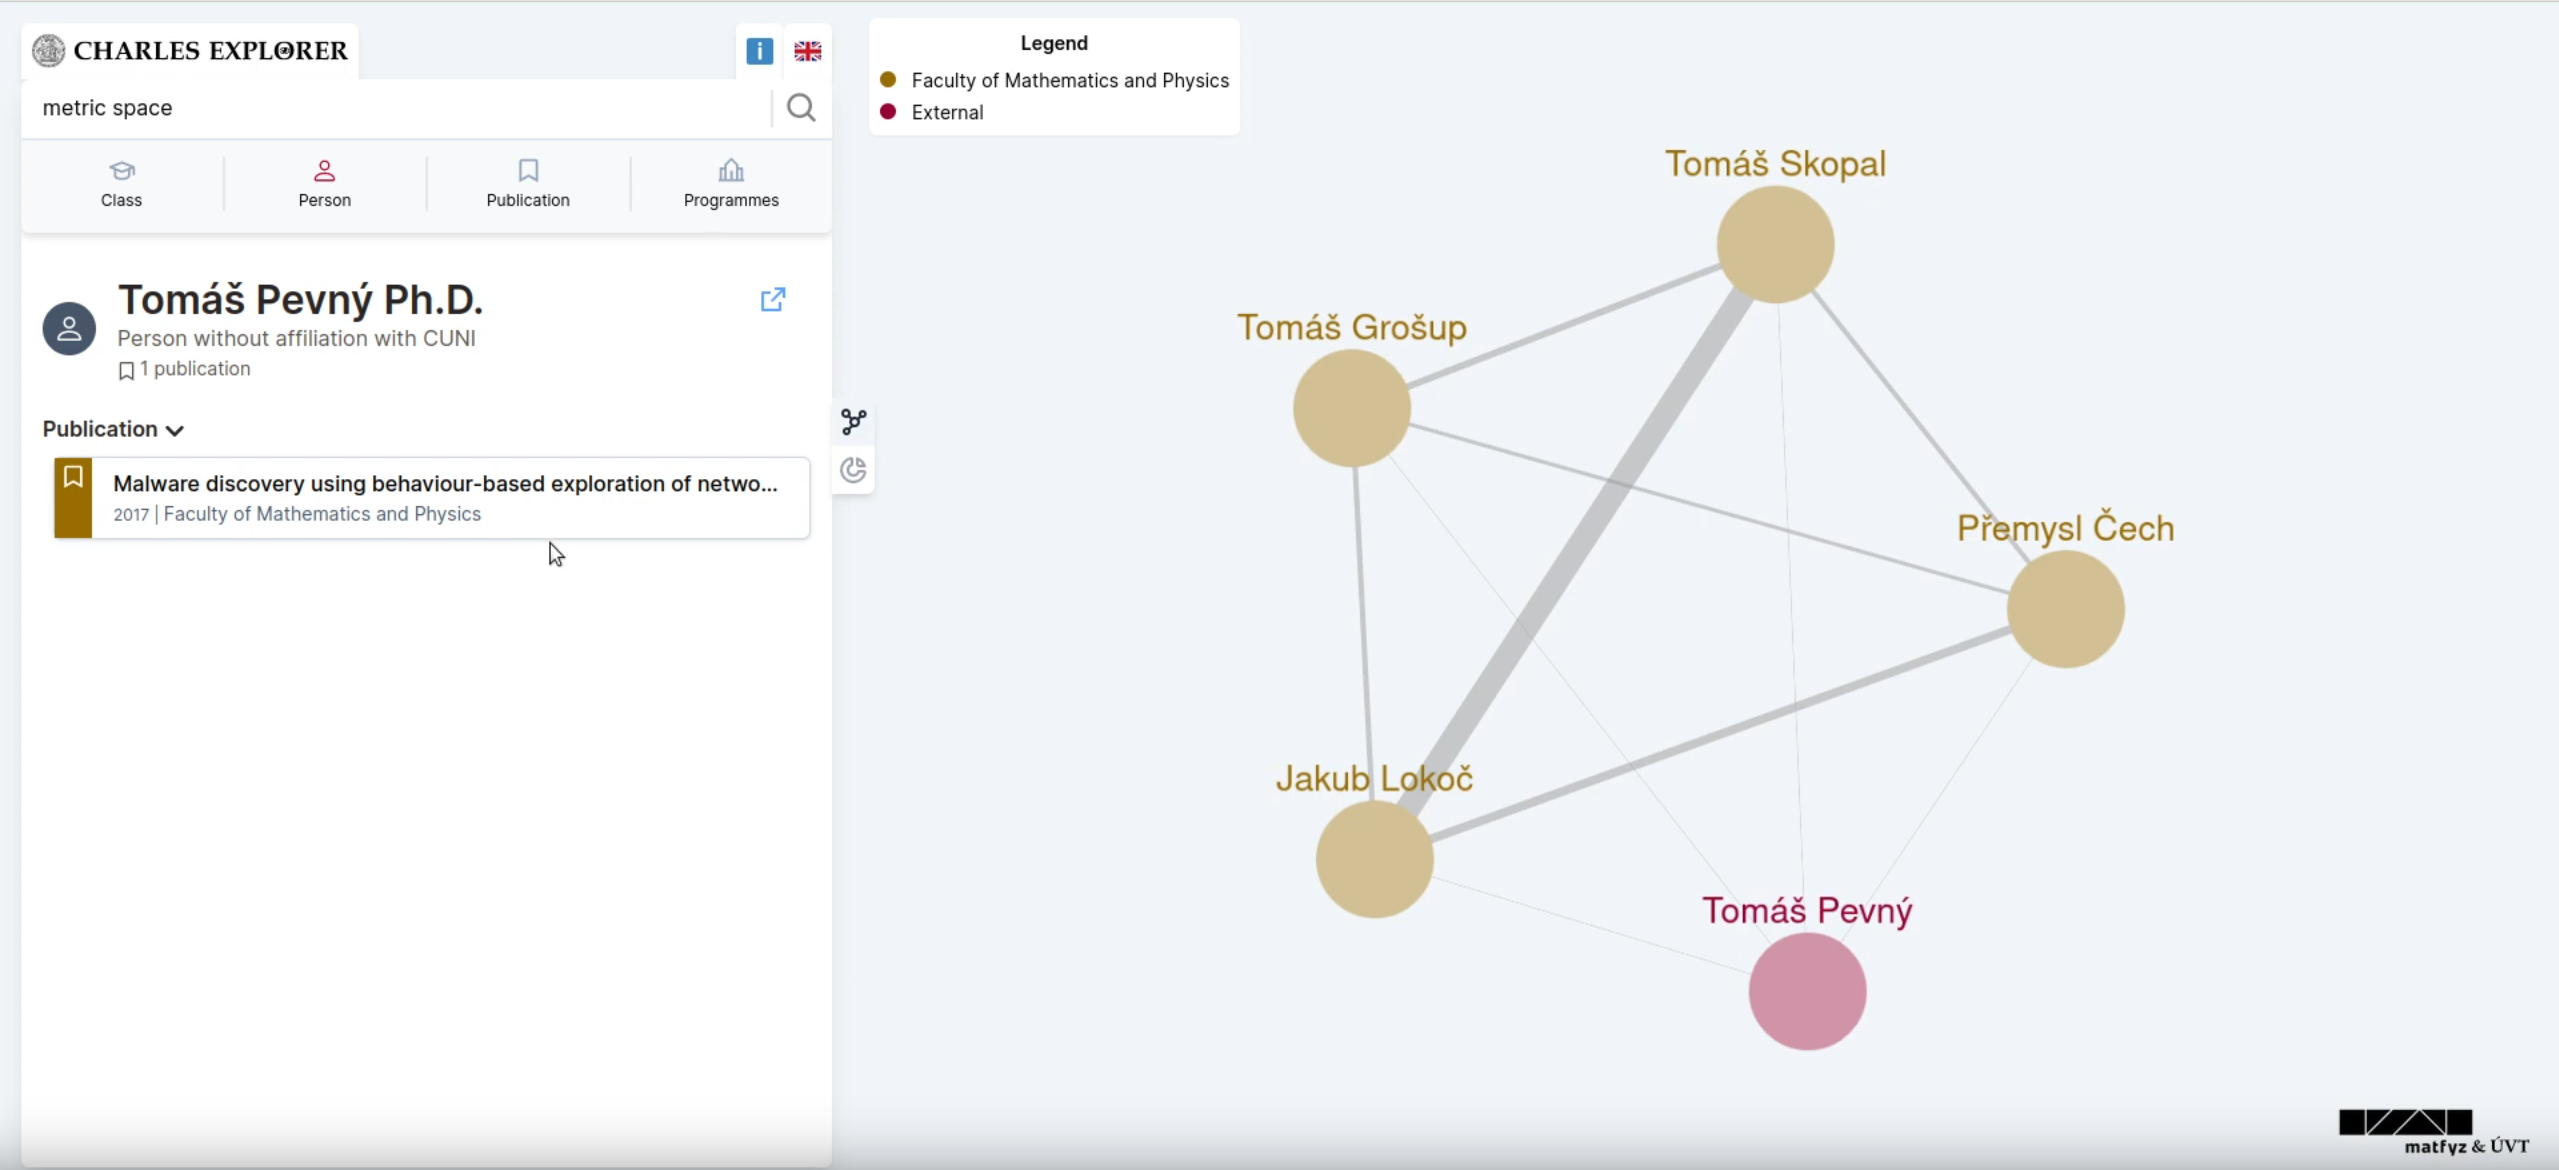
\includegraphics[width=0.8\textwidth]{../img/charles-explorer-old-view.png}
    \centering
    \caption{Charles Explorer showing the \textit{ego network} of a person.}
\end{figure}

The graph is displayed with a force-directed layout. The edge thickness is proportional to the number of common publications between 
the two people and the colors of the nodes represent the person's faculty association.

This approach has multiple drawbacks which we will now discuss.

\subsection{Problems with color coding} \label{sec:color-coding}

Firstly, the color coding of the nodes does not prove useful, as it hinders the \textit{visual decoding} of the graph.
The user spends attention on reading the legend rather than interpreting the graph subconsciously.

This is especially true for larger ego networks with many nodes with different faculty affiliations. 
Additionaly, the application does not provide any alternative visual cue for color vision deficient users.

\begin{figure}[ht!]
    \captionsetup{width=.9\linewidth}
    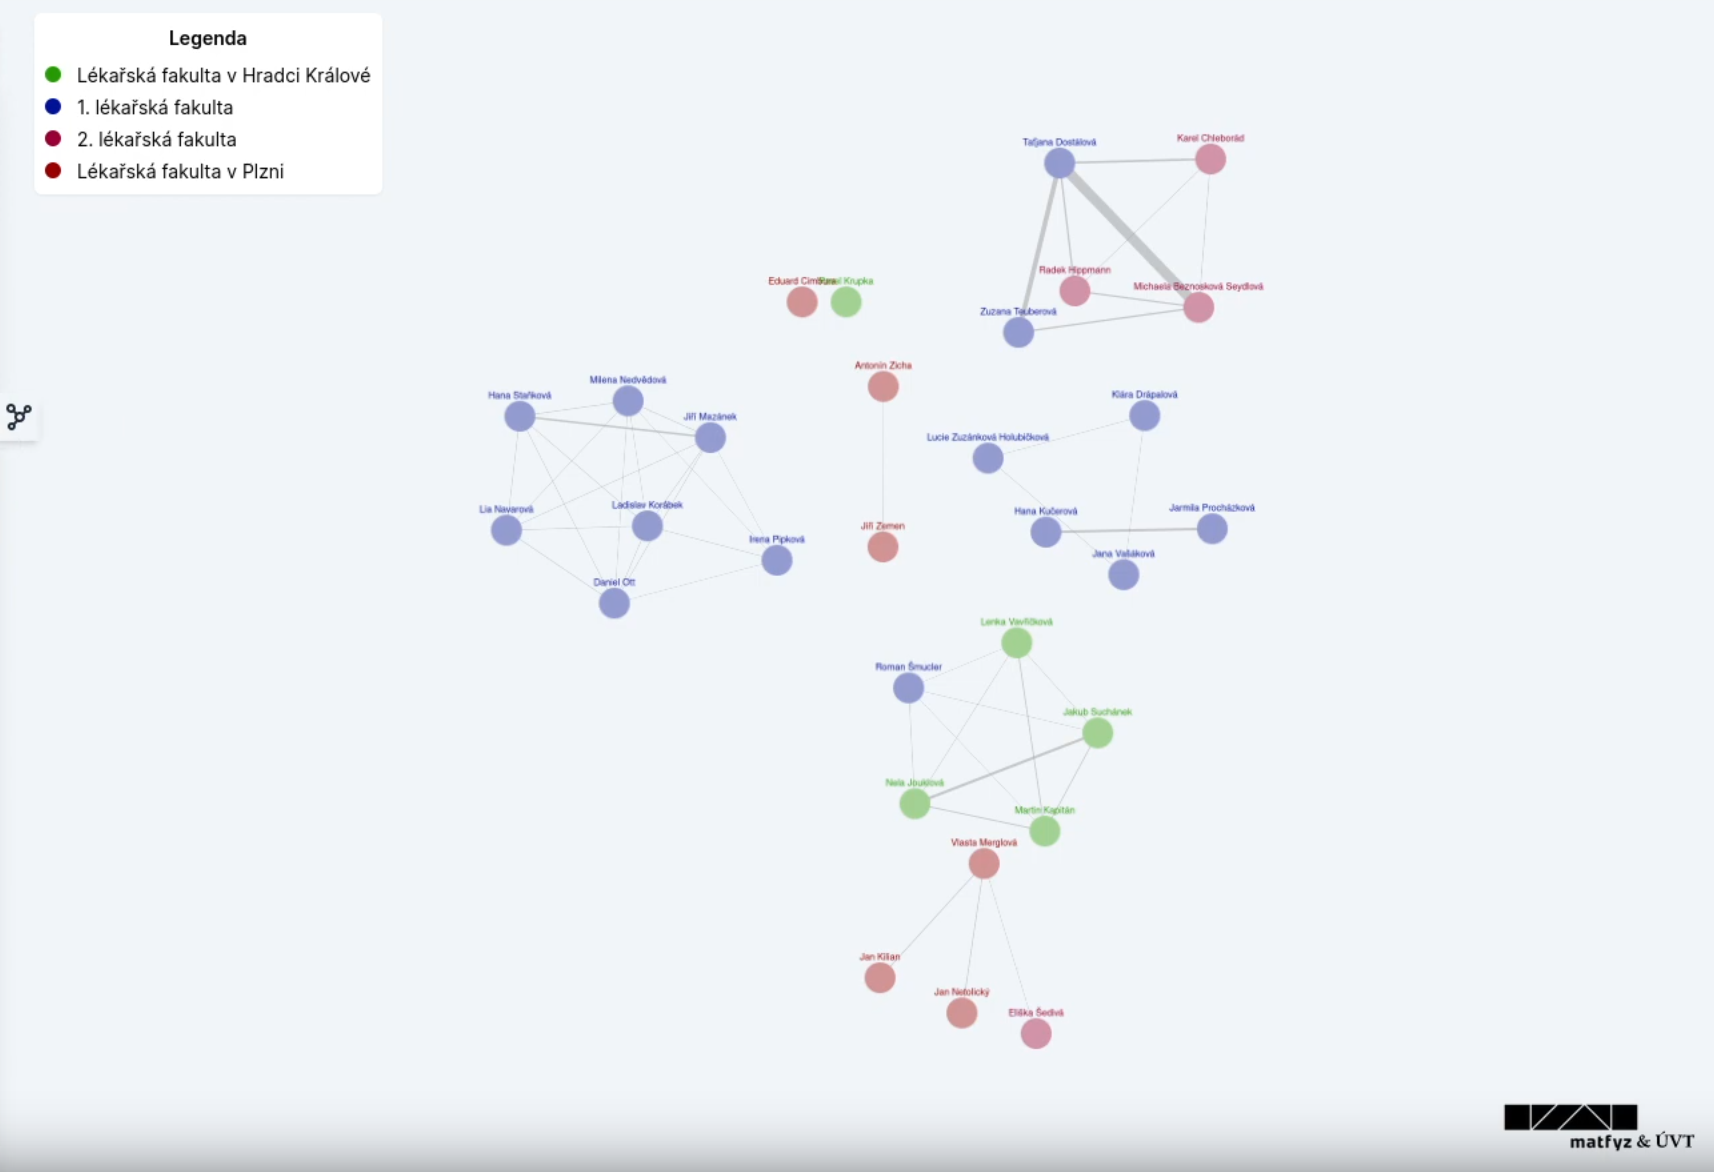
\includegraphics[width=0.7\textwidth]{../img/color-coding.png}
    \centering
    \caption{Graph view for query \textit{`dentistry'} shows nodes with various faculty affiliations.}
\end{figure}

According to \cite{Cleveland1985}, the upper bound on color discrimination in one figure is 5–6 colors for a healthy viewer. 
This is not enough for the 17 faculties and departments of Charles University. 
With faculties, there is also little room for a meaningful aggregation (of more faculties into one color), as the faculty structure is not hierarchical.

\subsection{Layouting problems} \label{sec:layouting-problems}

The arbitrary positions of the nodes based on the physical simulation layout increase the cognitive load 
of the viewer and contribute to the graph's worse readability.

\cite{munzner2015visualization} states that the position of data points on a common scale is the most effective way to communicate the data to the viewer.
By using the physical simulation layout, we are willingly giving up this visual channel (the \texttt{x} and \texttt{y} position of the nodes in the screen space).

In case the user is looking for a specific person in the graph, they have to scan the whole graph to find the person, as the node position does not code any inherent information about the person.

\subsection{Contracting publication nodes into edges}

The current data visualization effectively presents a monopartite projection of the social network - uses authors as the nodes and contracts publications as the edges.
The number of common publications is aggregated to the edge thickness. \cite{10.5555/2385879} considers thickness a visual channel with a limited quantitative resolution.

Setting the edge width in proportion to the number of common publications might also cause confusion, as the \textit{area} of the edge depends both on the width and the length of the edge.
Longer edges might appear more important than the shorter ones, even though they might denote the same number of common publications.

This is undesirable, as it goes against the underlying idea of the physical simulation layout, which places the nodes closer to each other if they are more connected.

Furthermore, the contraction of the publication nodes into edges poses another problem.
A publication with $n$ authors contributes to $\frac{n(n-1)}{2}$ edges between its authors. 

\begin{figure}[ht!]
    \captionsetup{width=.9\linewidth}
    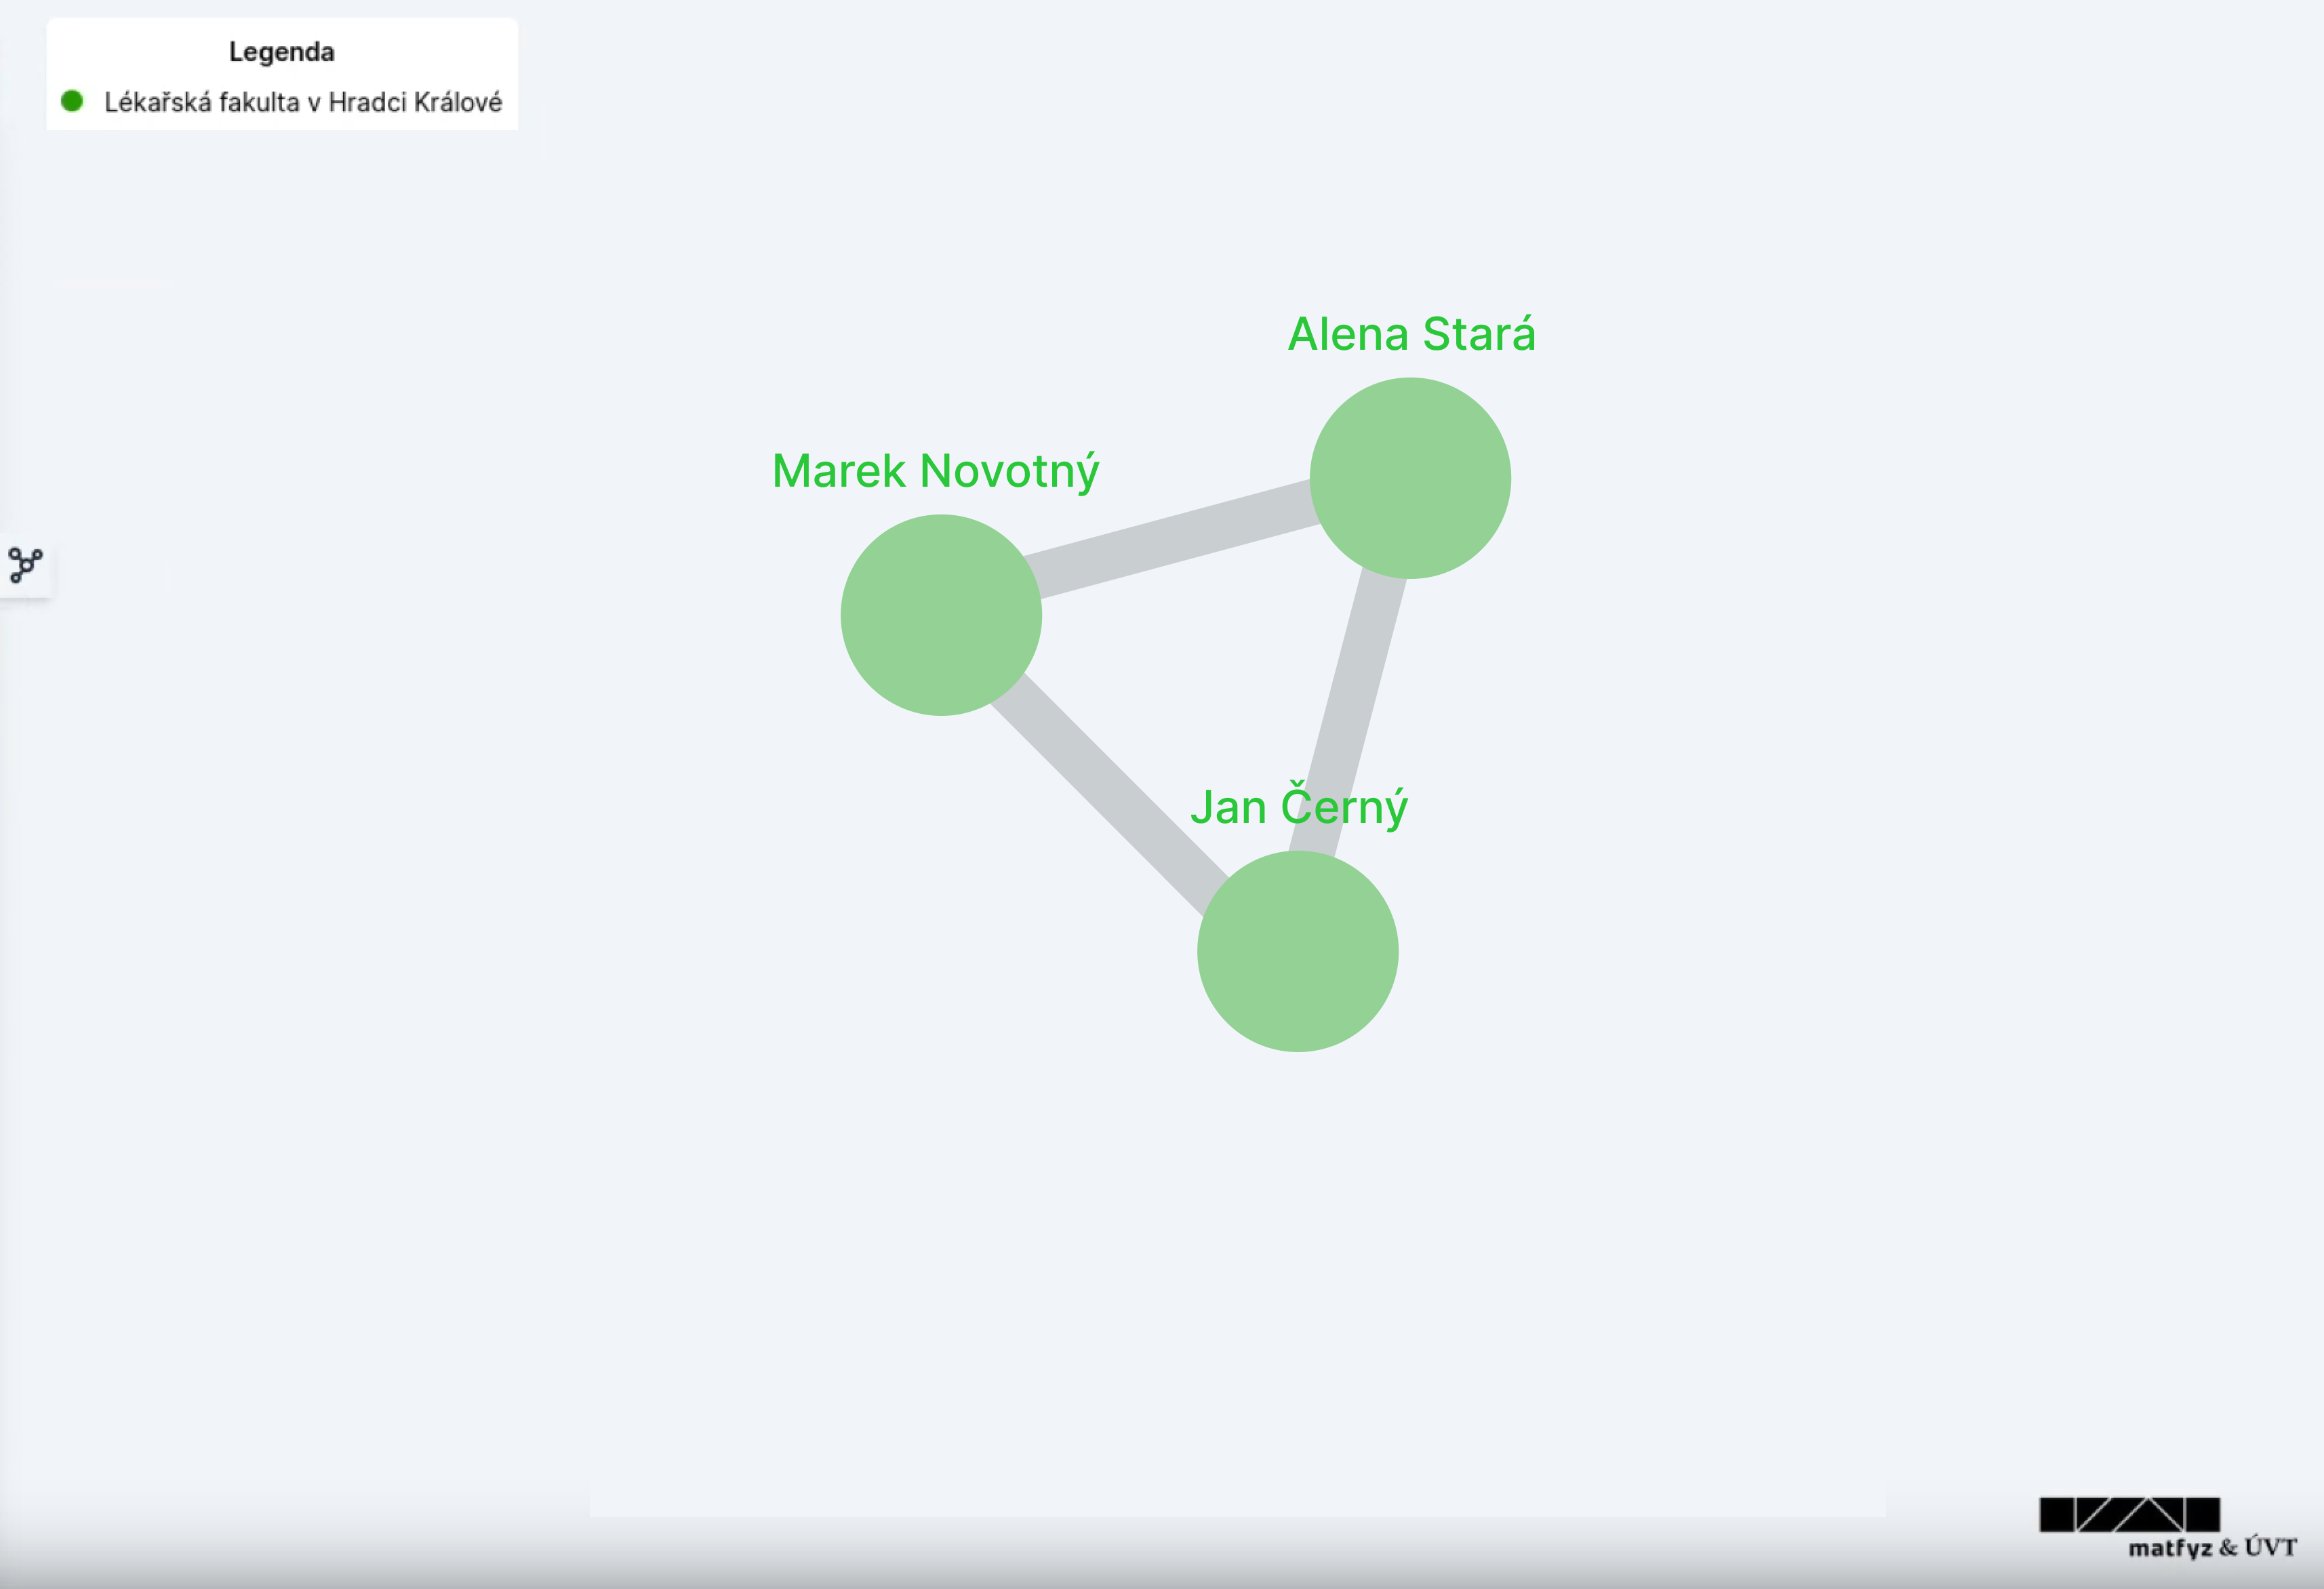
\includegraphics[width=0.7\textwidth]{../img/contraction.png}
    \centering
    \caption{The monopartite projection correctly shows only coauthorship between pairs of authors. Larger communities of coauthors (\# coauthors > 2) are not displayed correctly in the graph.}
\end{figure}

This means that publications with one author are not represented in the graph at all, as there are no edges to draw between the nodes.

For publications with more than two authors, one publication is represented by multiple edges between all the pairs of the authors.
This clutters the graph with edges and makes the publication-edge mapping less readable. 
For correct representation of those publications, we would need to draw hyperedges between the nodes, which might cause the readability of the graph to decrease even further.

\section{Addressing the issues}\label{sec:addressing-issues}

To address the problems from the section \ref{sec:current-state} and improve the visualization of the ego networks, we propose changes to the current visualization.
We also implement an experimental prototype visualization of the proposed changes.

\subsection{Ego-network visualization}

To start, we can address the problem of the \textit{publication-edge contraction} by displaying the publications as nodes in the graph.

This way, both the entity types (authors and publications) are displayed as \textit{nodes} in the visualization.
This is perhaps easier to understand for a layman, as both authors and publications are real-life entities. 
The edges between the nodes now represent an incidence relation between the two entities.

The resulting graph is a bipartite graph, with two types of nodes - authors and publications, and edges connecting the authors to the publications they have co-authored.

To support the \textit{visual decoding} of the graph, we distinguish the two types of nodes by their shape. 
This way, the user can easily distinguish between the authors and the publications, even if they are color-vision deficient 
or are viewing the visualization reproduced using a monochrome display medium (for example a print from a black-and-white printer).

The main node (the ego) is highlighted with color fill - since it is the only node of this type in the graph,
it is easy to distinguish from the other nodes - even with monochrome display mediums or color vision impairments.

\begin{figure}[ht!]
    \captionsetup{width=.9\linewidth}
    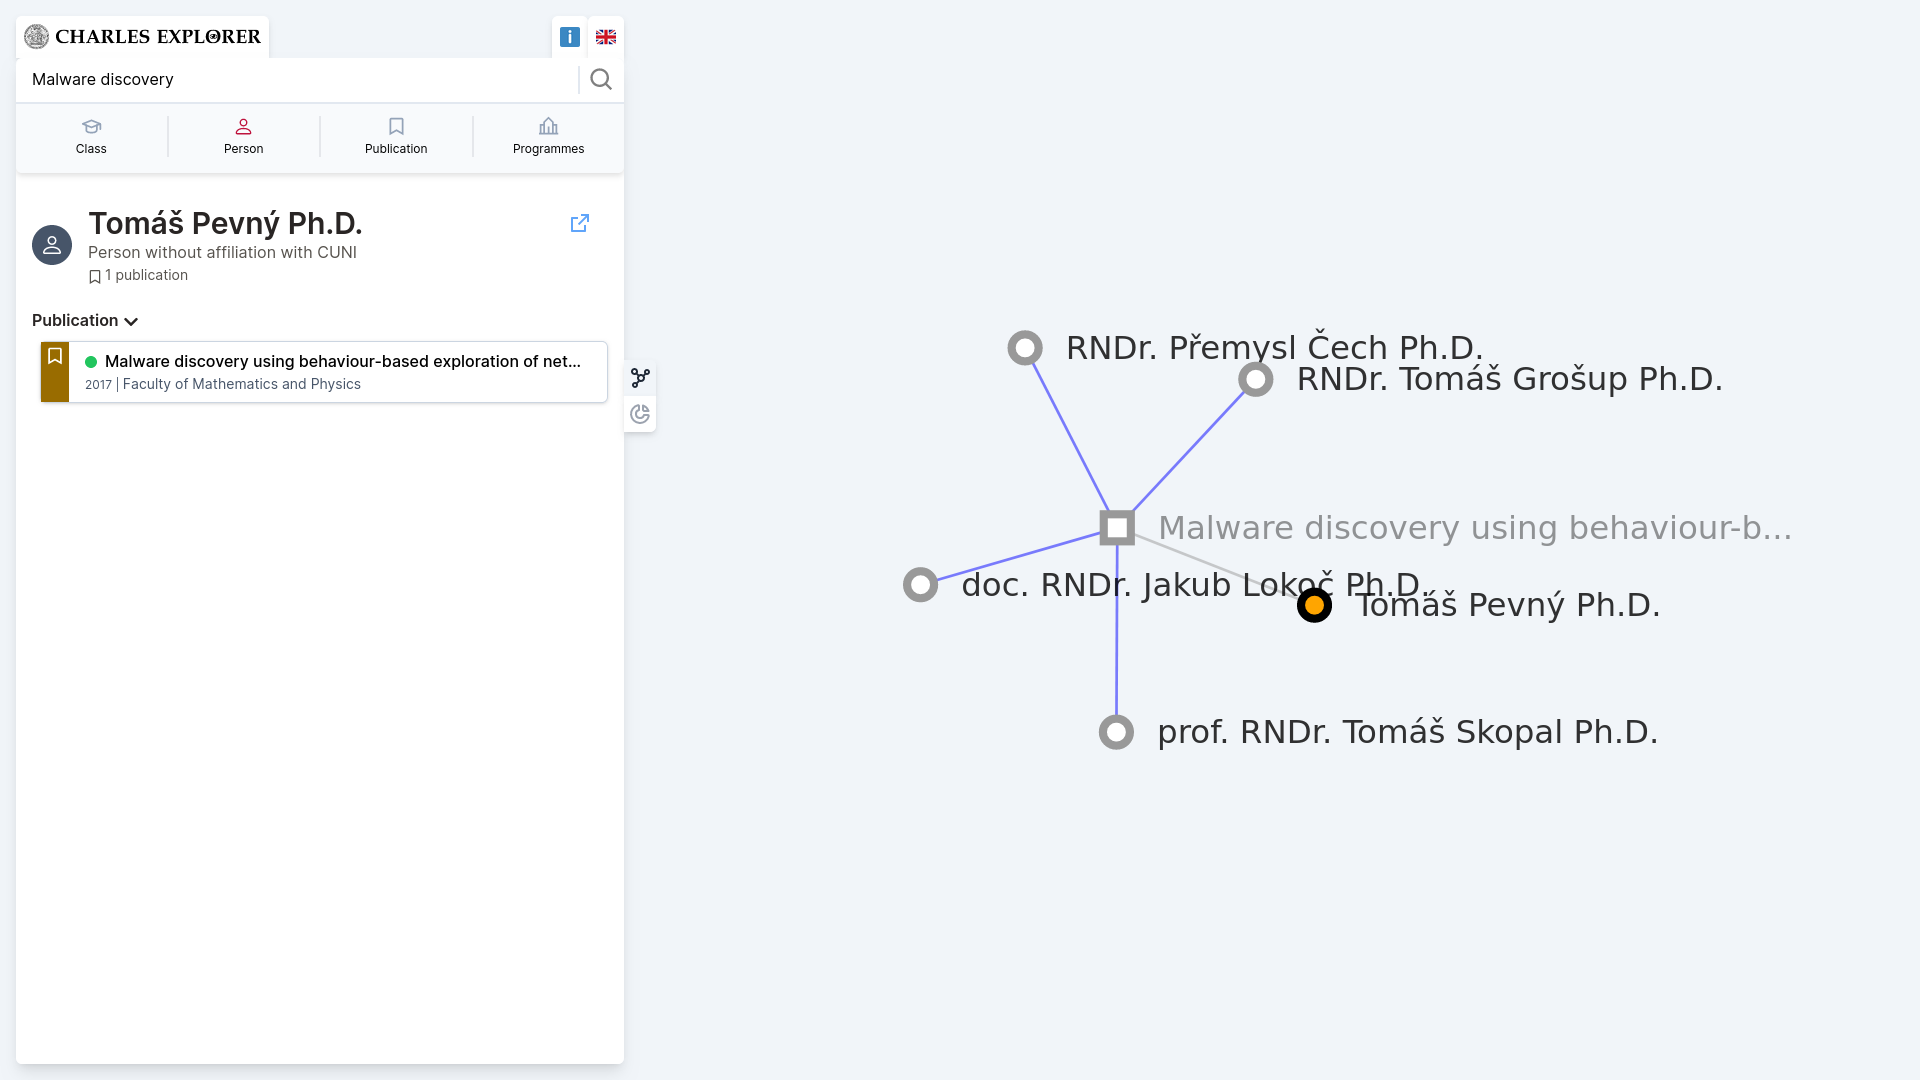
\includegraphics[width=0.7\textwidth]{../img/publications-and-people.png}
    \centering
    \caption{In the proposed visualization, the publications are displayed as nodes in the graph. \textit{Larger-than-binary} coauthorships are now represented correctly.}
\end{figure}

This approach also removes the need for the edge-width encoding of the number of common publications.

To avoid the color coding problems from \ref{sec:color-coding}, we defer the faculty affiliation information to the node tooltip.
This is only visible after the user hovers over the node with the mouse cursor, so it does not clutter the graph view.

\subsection{Node locality and layouting}

As mentioned in \ref{sec:layouting-problems}, the arbitrary positions of the nodes in the force-directed layout increase the cognitive load of the viewer.
For larger graphs, the viewer might not be able to find the node they are looking for, as the node position does not code any inherent information about the person.

To address this, we propose a search tool that highlights the search results in the graph.

\begin{figure}[ht!]
    \captionsetup{width=.9\linewidth}
    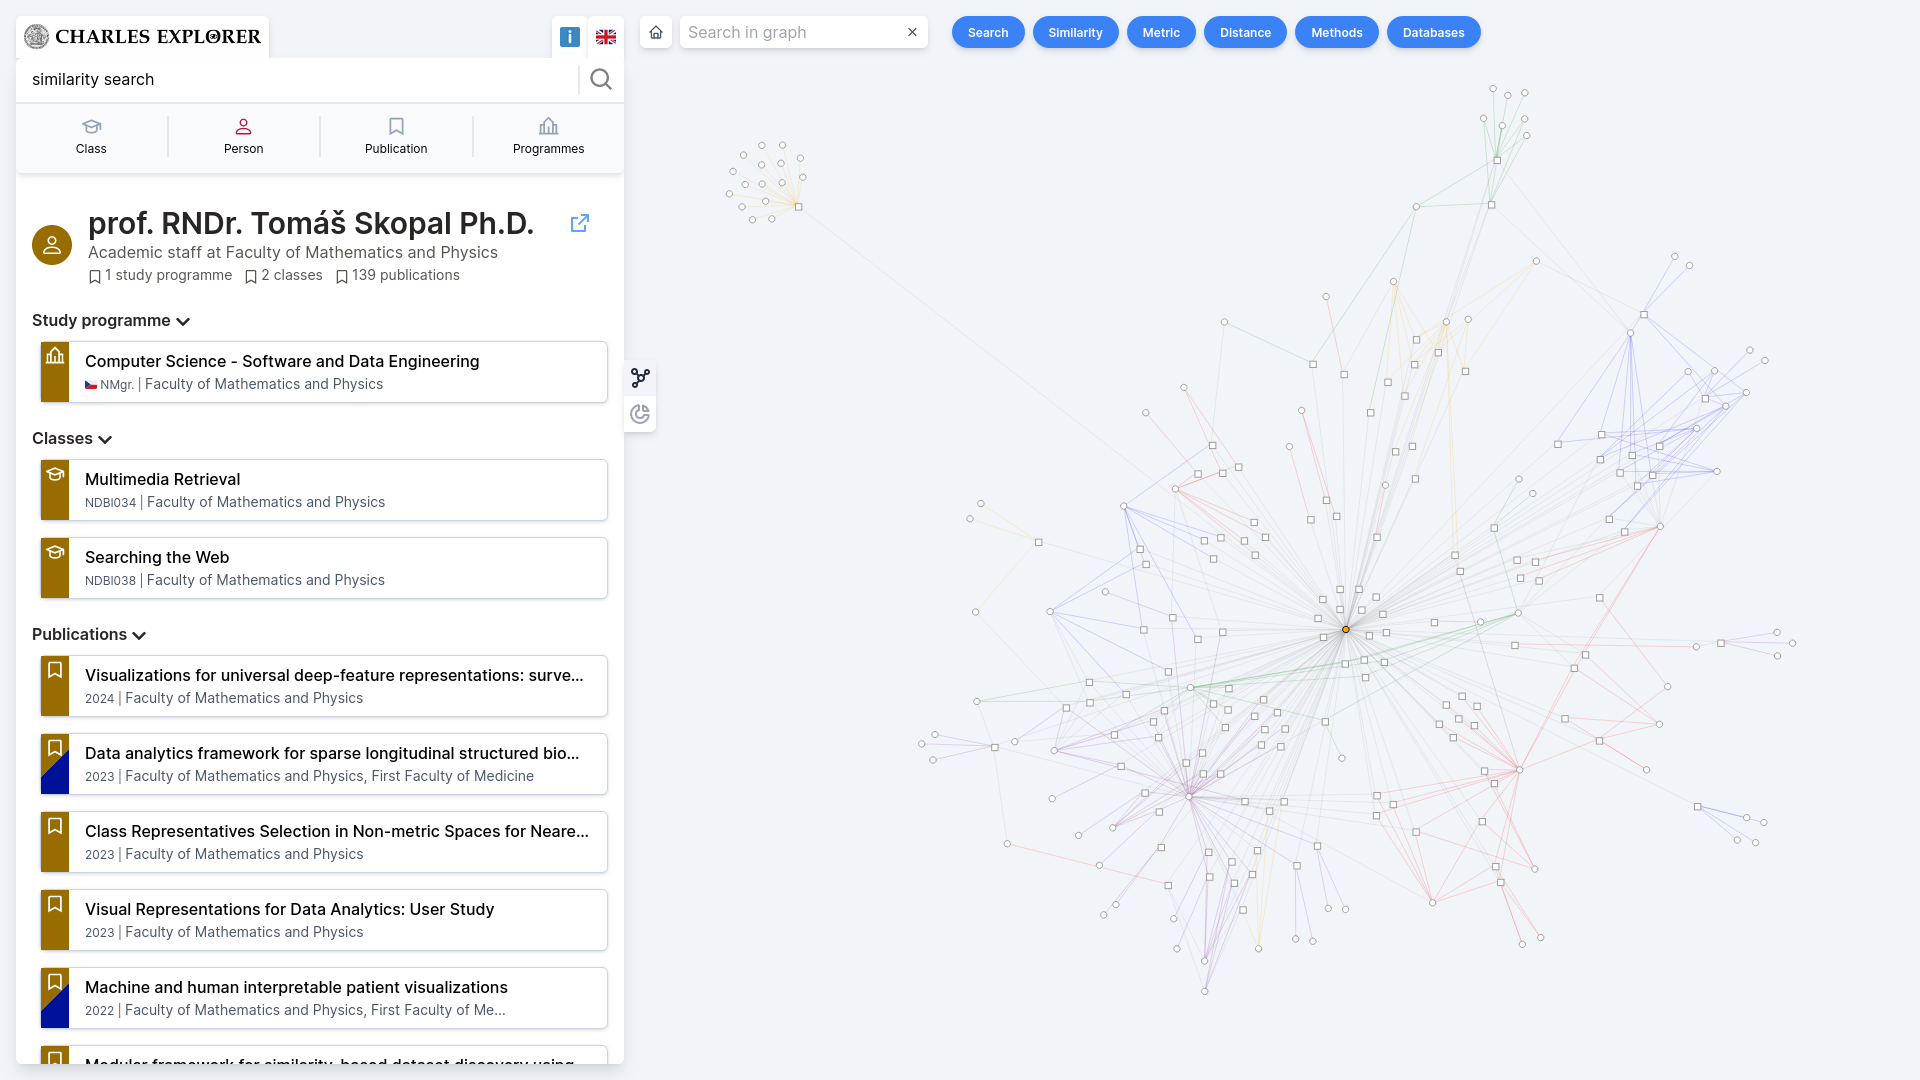
\includegraphics[width=0.8\textwidth]{../img/big-network.png}
    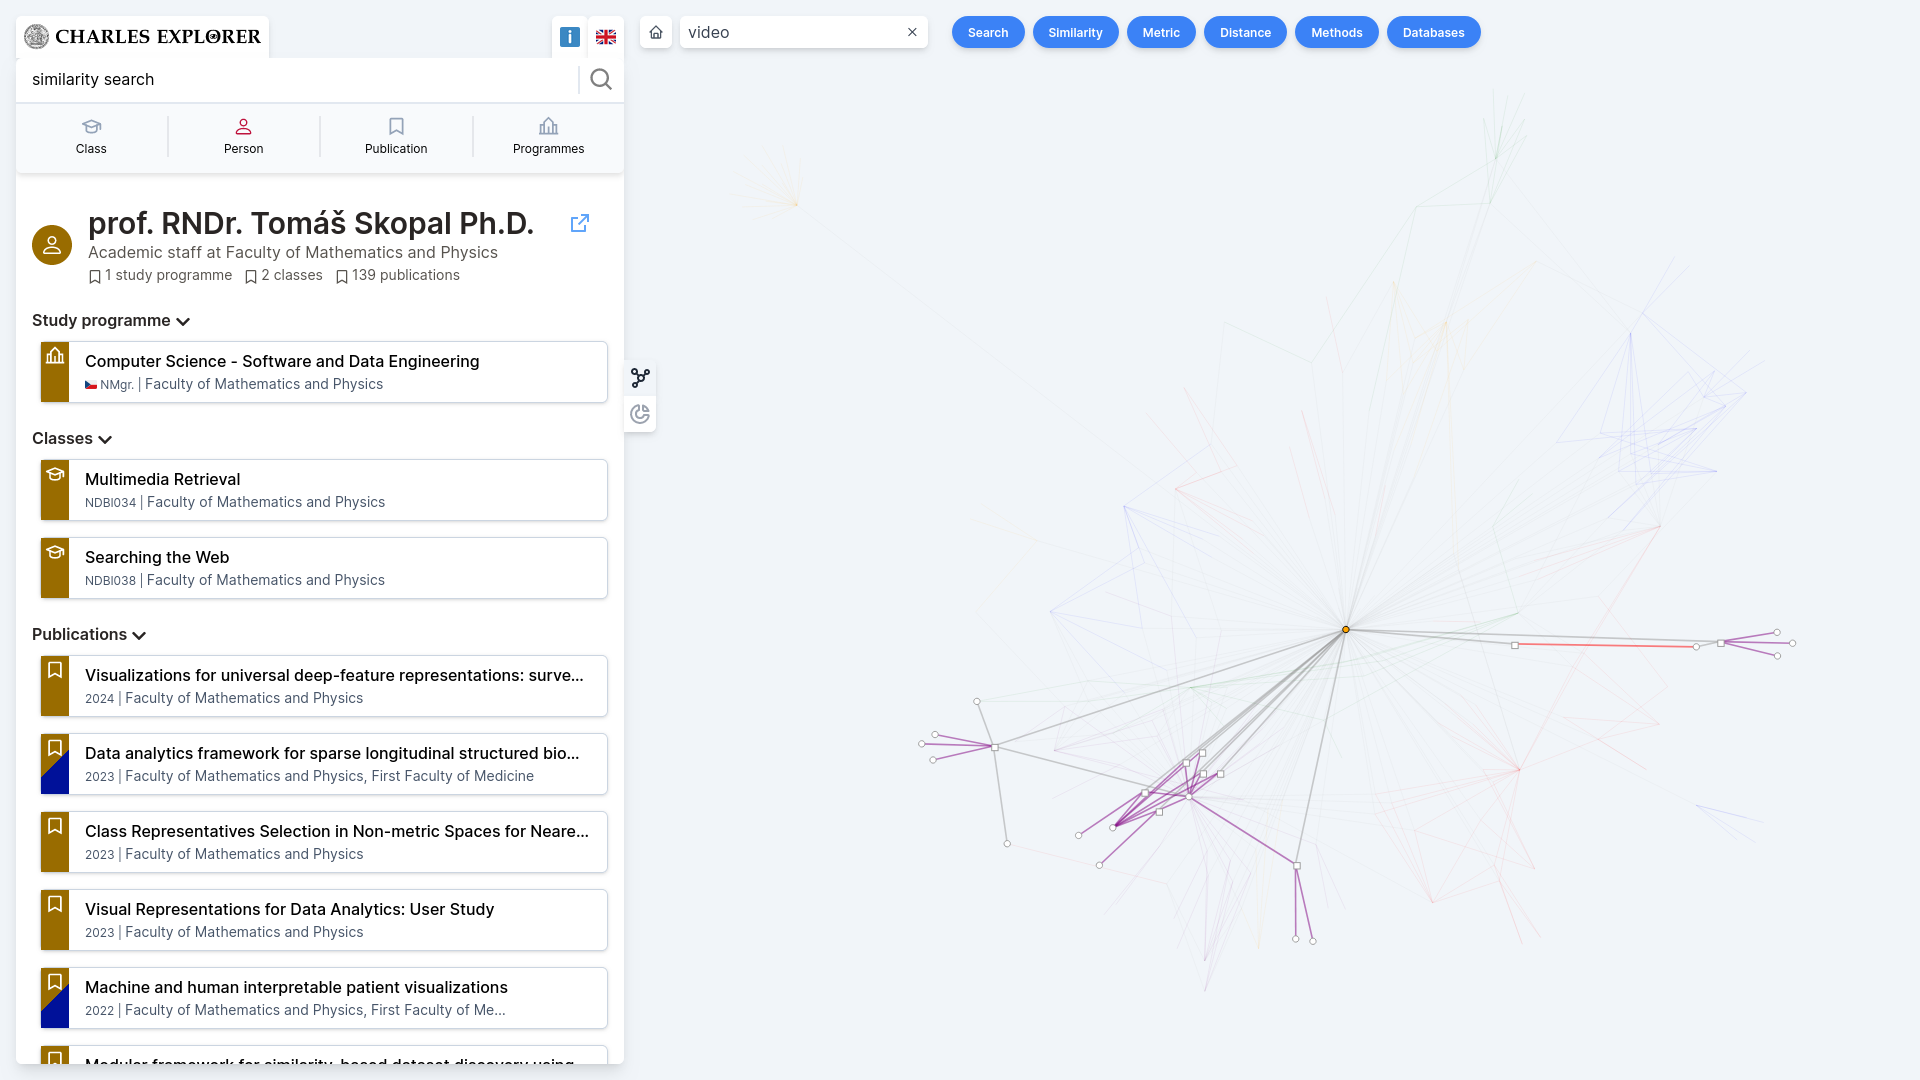
\includegraphics[width=0.8\textwidth]{../img/big-network-search.png}
    \centering
    \caption{The first picture shows a large ego network with many nodes. The second picture shows the same network with entities highlighted by the search tool (search for \textit{video} shows related publications and co-authors).}
\end{figure}

To further improve the graph readability and the usability of the tool, we propose a \textit{query suggester}. 
This is a user interface element consisting of multiple buttons with predefined queries, which the user can click to search for the query in the graph.
The suggested queries are based on tf-idf analysis of the text data connected to the ego network (publication titles and abstracts). 

The tokens (unigrams and bigrams) with the highest tf-idf score are selected as the suggested queries.

\subsection{Faculty affiliation}

While we have already addressed the color coding issues from \ref{sec:color-coding} by introducing the on-hover tooltip, 
this has removed some of the information from the graph view.

In the original visualization, the faculty affiliation for people was displayed as the node color.
This has helped the user to quickly identify the faculty affiliation of the ego's collaborators, 
but also to see the distribution of the faculty affiliations in the ego network, 
and identify interesting collaboration patterns. 
This is no longer possible with the new tooltip-based approach.

To address this, we propose a new visualization of the faculty affiliation data.
Each co-author of the ego has a faculty affiliation assigned to them, along with the number of common publications with the ego.

For visualizing the distribution of faculty affiliations in the ego network, we can use a \textit{pie chart}.

\begin{figure}[ht!]
    \captionsetup{width=.9\linewidth}
    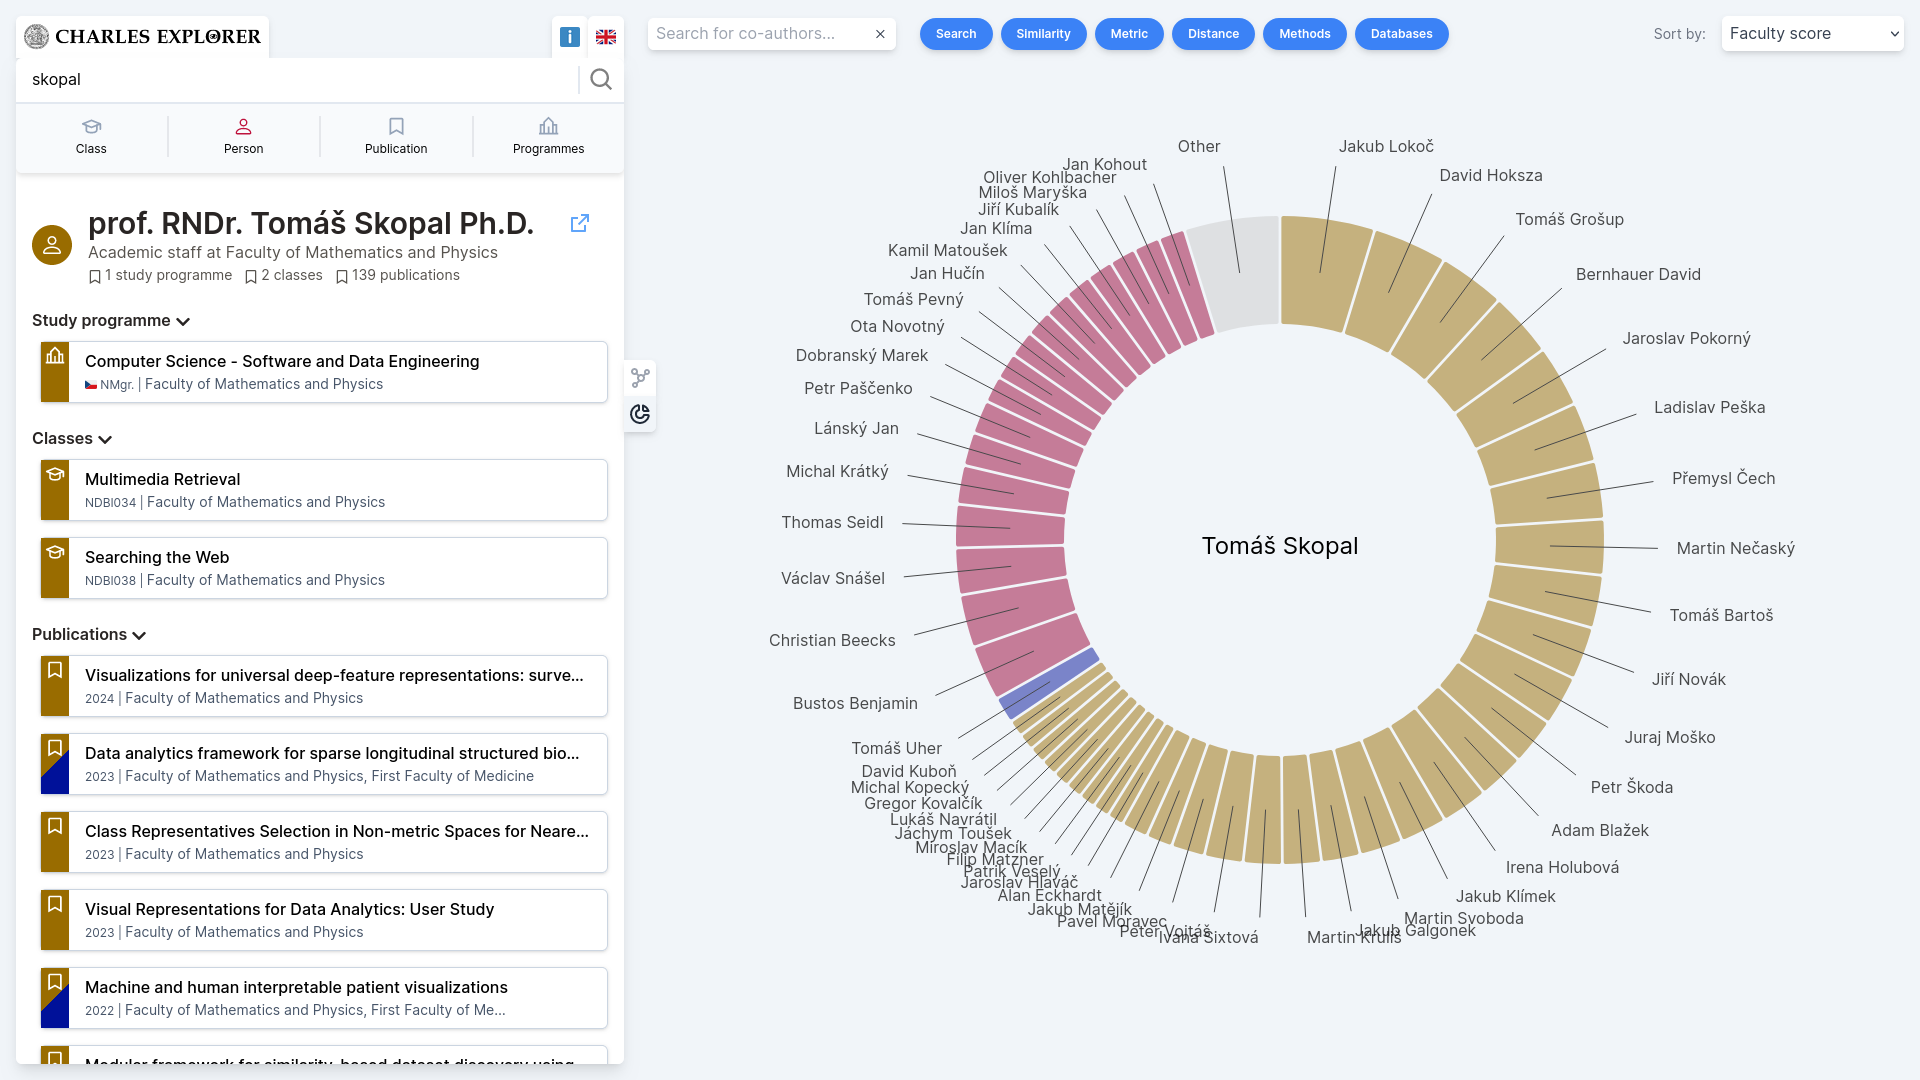
\includegraphics[width=0.8\textwidth]{../img/pie-chart.png}
    \centering
    \caption{The \textit{pie chart} view shows the distribution of faculty affiliations in the ego network, as well as the most frequent collaborators of the ego.}
\end{figure}

This visualization is still suffering from some of the problems of the original one. 

A publication with $n$ authors still contributes to $(n-1)$ pie chart arcs. 
This causes the solo publications to not be represented in the pie chart at all, and the publications with more than two authors to be overrepresented.

The color coding of the pie chart arcs (denoting the faculty affiliation) is also not ideal since it still poses a problem for color-vision deficient users.

To address these issues, we add a few more features to the pie chart view.

Firstly, we reuse the tooltip user interface element from the graph view. 
When the user hovers over the pie chart arc, they can see the faculty affiliation name and the number of co-authored publications.

This helps both the color vision deficient users with identifying the faculty affiliation, and the general users with understanding the scale of the collaboration.

Secondly, we add an on-click boolean \texttt{AND} filter. 
When the user clicks on the pie chart arc, the view filters the underlying data to only represent co-authors of both the ego and the clicked-on co-author.

\begin{figure}[ht!]
    \captionsetup{width=.9\linewidth}
    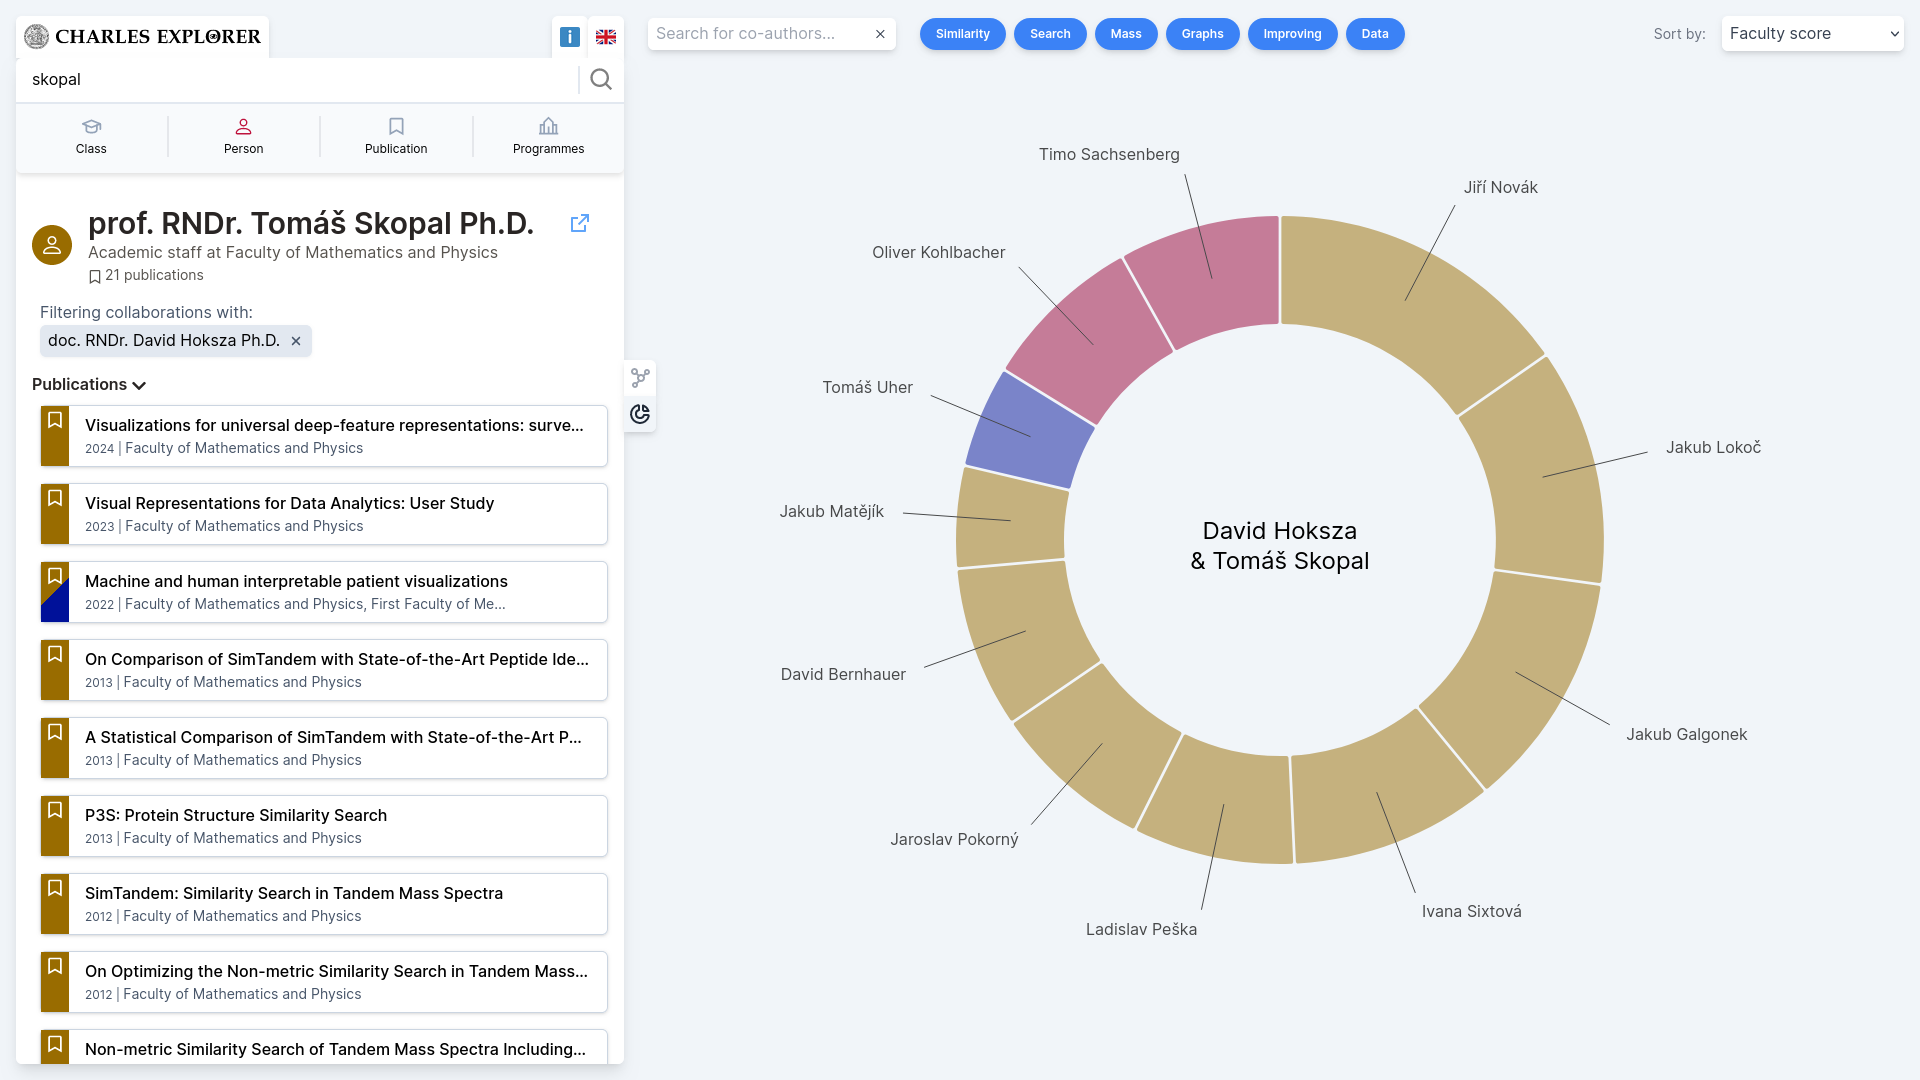
\includegraphics[width=0.8\textwidth]{../img/pie-chart-filter.png}
    \centering
    \caption{Right-clicking on the pie chart arc shows the intersection of the ego's and the clicked-on person's collaborators.}
\end{figure}

The \texttt{AND} filter can be used repeatedly, adding new ``pinned'' collaborators one at a time.
Focusing on a smaller subset of the ego network can help to mitigate the problems with the overrepresentation of the publications with more than two authors
helping the user to understand the smaller-scale collaboration patterns better.

The filter also applies to the left side of the view, where the user can see the actual publications of the selected co-authors.
This further clears up the multiple co-authorship problem.



\chapter*{Conclusion}
\addcontentsline{toc}{chapter}{Conclusion}

The conclusion wraps up the thesis, describing the achievements we've reached and suggests ideas for further research.

\dots

%%% Bibliography
%%% Bibliography (literature used as a source)
%%%
%%% We employ bibTeX to construct the bibliography. It processes
%%% citations in the text (e.g., the \cite{...} macro) and looks up
%%% relevant entries in the bibliography.bib file.
%%%
%%% The \bibliographystyle command selects, which style will be used
%%% for references from the text. The argument in curly brackets is
%%% the name of the corresponding style file (*.bst). Both styles
%%% mentioned in this template are included in LaTeX distributions.

\bibliographystyle{plainnat}    %% Author (year)
% \bibliographystyle{unsrt}     %% [number]

\renewcommand{\bibname}{Bibliography}

%%% Generate the bibliography. Beware that if you cited no works,
%%% the empty list will be omitted completely.

\bibliography{bibliography}

%%% If case you prefer to write the bibliography manually (without bibTeX),
%%% you can use the following. Please follow the ISO 690 standard and
%%% citation conventions of your field of research.

% \begin{thebibliography}{99}
%
% \bibitem{lamport94}
%   {\sc Lamport,} Leslie.
%   \emph{\LaTeX: A Document Preparation System}.
%   2nd edition.
%   Massachusetts: Addison Wesley, 1994.
%   ISBN 0-201-52983-1.
%
% \end{thebibliography}


%%% Figures used in the thesis (consider if this is needed)
\listoffigures

%%% Tables used in the thesis (consider if this is needed)
%%% In mathematical theses, it could be better to move the list of tables to the beginning of the thesis.
\listoftables

%%% Abbreviations used in the thesis, if any, including their explanation
%%% In mathematical theses, it could be better to move the list of abbreviations to the beginning of the thesis.
\chapwithtoc{List of Abbreviations}
\printacronyms[
	heading=none,
	display=used,
	sort=true,
]


%%% Attachments to the master thesis, if any. Each attachment must be
%%% referred to at least once from the text of the thesis. Attachments
%%% are numbered.
%%%
%%% The printed version should preferably contain attachments, which can be
%%% read (additional tables and charts, supplementary text, examples of
%%% program output, etc.). The electronic version is more suited for attachments
%%% which will likely be used in an electronic form rather than read (program
%%% source code, data files, interactive charts, etc.). Electronic attachments
%%% should be uploaded to SIS and optionally also included in the thesis on a~CD/DVD.
%%% Allowed file formats are specified in provision of the rector no. 72/2017.

% \appendix
% \chapter{Attachments}

% \section{First Attachment}

\openright
\end{document}
